\documentclass[brazil,ruledheader]{abntifes}
%\documentclass[brazil,twoside,ruledheader]{abntifes}
\usepackage[T1]{fontenc}
%\usepackage[latin1]{inputenc}
\usepackage[utf8]{inputenc}
\usepackage[brazil]{babel}
\usepackage[]{algorithm2e}
\usepackage{pslatex}
\usepackage{url}
\usepackage{fancyhdr}
\usepackage{graphicx}
\usepackage{amsmath, amsthm, amssymb}
\usepackage{exercise}
\usepackage{makeidx}
\usepackage{setspace}
\usepackage{multicol}    
\usepackage{upquote}
\usepackage{graphicx}
\usepackage{float}
\usepackage{epigraph}
\usepackage[]{mcode}
%%%%%%%%%%%%%%%%%%%%%%%%%
%\usepackage{indentfirst}
\graphicspath{{imagens/}}
\usepackage[]{listings}

\lstset{numbers=left, stepnumber=5, firstnumber=1, numberstyle=\tiny, extendedchars=true, breaklines=true, frame=tb, basicstyle=\footnotesize, stringstyle=\ttfamily, showstringspaces=false }

%\makenomenclature

% Para listar programas em C# 
\lstdefinelanguage{cs}
  {morekeywords={abstract,event,new,struct,as,explicit,null,switch
		base,extern,object,this,bool,false,operator,throw,
		break,finally,out,true,byte,fixed,override,try,
		case,float,params,typeof,catch,for,private,uint,
		char,foreach,protected,ulong,checked,goto,public,unchecked,
		class,if,readonly,unsafe,const,implicit,ref,ushort,
		continue,in,return,using,decimal,int,sbyte,virtual,
		default,interface,sealed,volatile,delegate,internal,short,void,
		do,is,sizeof,while,double,lock,stackalloc,
		else,long,static,enum,namespace,string, },
	  sensitive=false,
	  morecomment=[l]{//},
	  morecomment=[s]{/*}{*/},
	  morestring=[b]",
}

\newcommand{\AUTOR}{Oscar Neiva Eulálio Neto}
\newcommand{\SEGUNDOAUTOR}{}
\newcommand{\ORIENTADOR}{D.Sc. Eduardo Krempser da Silva}
\newcommand{\COORIENTADOR}{D.Sc. Marcos Garcia Todorov}
\newcommand{\TITULO}{Simulação de Algoritmos Distribuídos Aplicados ao Cálculo do \textit{PageRank}}
\newcommand{\CURSO}{Tecnólogo em Tecnologia da Informação e da Comunicação}
\newcommand{\GRAU}{Tecnólogo em Tecnologia da Informação e da Comunicação}
% \newcommand{\GRAU}{Tecnólogo em Análise e Desenvolvimento de Sistemas}
\newcommand{\INSTITUICAO}{Faculdade de Educação Tecnológica do Estado do Rio de Janeiro - FAETERJ/Petrópolis}
\newcommand{\ANO}{Outubro, 2016}
\newcommand{\DATA}{27 de Outubro de 2016}
\newcommand{\LOCAL}{Petrópolis - RJ}
\newcommand{\epigrafe}{\vspace{1cm}{\raggedright\par\sffamily\slshape\par}}
\begin{document}

\autor{\AUTOR}
\titulo{\TITULO}
\orientador{\ORIENTADOR}
\coorientador{\COORIENTADOR}

\comentario{Trabalho de Conclusão de Curso apresentado à Coordenadoria do Curso de \CURSO\
	    da \INSTITUICAO , como requisito parcial para obtenção do título de \GRAU .}

\instituicao{\INSTITUICAO}
\curso{\CURSO}
\governo{Governo do Estado do Rio de Janeiro}
\secretaria{Secretaria de Estado de Ciência e Tecnologia}
\fundacao{Fundação de Apoio à Escola Técnica}
\cpti{Centro de Educação Profissional em Tecnologia da Informação}
\local{\LOCAL}
\data{\ANO}

\capa

\folhaderosto

% Ficha Catalográfica
%\begin{figure}
%\includegraphics[width=11cm]{FichaCatalografica.pdf}
%\end{figure}

% Folha de Aprovação
\newpage
\vfill 
\null
\begin{center}
{\Huge {\bfseries\itshape Folha de Aprovação}}\\[3cm]
\begin{espacoduplo}
Trabalho de Conclusão de Curso sob o título \textit{``\TITULO''},
defendida por \AUTOR\ e aprovada em \DATA, em \LOCAL, pela banca examinadora constituída pelos
professores: \setlength{\ABNTsignthickness}{0.4pt}
\end{espacoduplo}
\setlength{\ABNTsignthickness}{0.4pt}

% ou inserir a página assinada e escaneada aqui
%\begin{figure}
%\includegraphics[]{Fo	lhaAprovacao.pdf}
%\end{figure}


\assinatura{Prof. \ORIENTADOR\\ Orientador \\ \INSTITUICAO}
\assinatura{Prof. \COORIENTADOR\\ Coorientador \\ Laboratório Nacional de Computação Científica - LNCC}  
\assinatura{Prof. M.Sc. Alberto Torres Angonese \\ \INSTITUICAO} 
%\assinatura{Prof. Banca Interna \\ \INSTITUICAO} 
%\assinatura{Prof. Banca Externa \\ Instituto do membro externo}

\end{center}


% Folha do Termo de Compromisso
\newpage

\vfill 
\null
\begin{center}
{\Huge {\bfseries\itshape Declaração de Autor}}\\[3cm]
\begin{espacoduplo}
Declaro, para fins de pesquisa acadêmica, didática e tecnico-científica, que o presente Trabalho de Conclusão
de Curso pode ser parcial ou totalmente utilizado desde que se faça referência à fonte e aos autores.
\end{espacoduplo}
\setlength{\ABNTsignthickness}{0.4pt}
\assinatura{\AUTOR}
Petrópolis, em \DATA
\end{center}


\chapter*{Agradecimentos}
Aos meus pais Oscar Filho e Márcia Nunes pelo apoio aos meus estudos, mesmo de longe durante os últimos anos. As minhas irmãs e familiares que de alguma forma durante esse período também me apoiaram.

Ao meu orientador de Iniciação Científica, professor Marcos Todorov, pelas orientações aos meus trabalhos no Laboratório Nacional de Computação Científica - LNCC, que resultaram na produção desta monografia.

Aos professores Eduardo Krempser e Alberto Angonese pelas orientações aos meus trabalhos no Laboratório de Sistemas Inteligêntes e Robótica - SIRLab.

Aos amigos do LNCC e do SIRLab, em especial a: Caio Graciani, Johnathan Fercher e Lucas Borsatto, pelo apoio e ajuda durante os meus estudos em sistemas e controle.

A todos os amigos, professores e funcionários da FAETERJ-Petrópolis e do LNCC que de alguma forma deram contribuições a minha formação. 
\vfill 
\null

\vspace{10cm}
\begin{center}
{\Huge {\bfseries\itshape Epígrafe}}\\[3cm]
\vspace{10cm}
\end{center}

%\begin{espacoduplo}
%\end{espacoduplo}


\epigraph{"A natureza é um templo augusto, singular,\\ 
		Que a gente ouve exprimir em língua misteriosa;\\
		Um bosque simbolista onde a árvore frondosa\\
		Vê passar os mortais, e segue-os com o olhar."}{(Charles Baudelaire)}

%\vspace{10cm}

\begin{resumo}
Desde o início das pesquisas no desenvolvimento de ferramentas de busca em 1994, os algoritmos responsáveis pelo ranqueamento de um conjunto de documentos interligados têm sido a parte mais desafiadora na implementação desses sistemas. Dentre esses algoritmos, o \textit{PageRank} do Google obteve grande destaque no final dos anos 90, fazendo com que cada vez mais o buscador fosse uma ferramenta indispensável na navegação pela \textit{Web}. Neste trabalho são apresentados os resultados obtidos das simulações dos modelos responsáveis pelo cálculo do \textit{PageRank}.

%Neste trabalho foram estudados os modelos e os problemas por trás da simulação do \textit{PageRank}.

%De tal forma que antes foi necessário estudar conceitos de sistemas dinâmicos, sistemas estocásticos e sistemas sujeitos a saltos, para que em seguida fosse feita uma revisão dos ultimos modelos propostos para o algoritmo na literatura. E por fim, implementadas as simulações desses modelos e analisados os resultados obtidos.
\end{resumo}

%\begin{abstract}
%Resumo em inglês ... "Não é obrigadorio"
%\end{abstract}
\listoffigures

%\listoftables

%Lista de abreviaturas

\tableofcontents{}


%%%%%%%%%%%%%%%%%%%%%
\chapter{Introdução}%
%%%%%%%%%%%%%%%%%%%%%

%Primeira Parte - Breve Historico e Revisão Bibliográfica 
A crescente quantidade de informação na \textit{Web} nos últimos anos, fez das ferramentas de busca algo indispensável na coleta de informação. O algoritmo \textit{PageRank} é a técnica chave do Google, proposta inicialmente em \cite{brin2012reprint} no ano de 1998. O Google é um dos mais bem sucedidos buscadores e o \textit{PageRank} é com certeza um dos fatores deste sucesso.

É possível encontrar na literatura artigos recentes \cite{lei2015distributed,ishii2014pagerank} que ilustram o crescente interesse da comunidade de sistemas e controle no tema. Tal interesse advém das diversas dificuldades que são encontradas no cálculo do \textit{PageRank}, devido a sua complexidade. O problema é de grande dimensão e em geral trata-se de um sistema com variações abruptas em sua estrutura. Além disso, a variabilidade da \textit{Web} torna necessária a atualização frequente do cálculo. Ademais, a possibilidade do cálculo ser efetuado através de recursos computacionais distribuídos \cite{ishiiTAC12} evidencia o caráter desafiador deste problema.

Para o cálculo do \textit{PageRank} algumas considerações devem ser feitas e um fator crítico a ser levado em conta é o tamanho da estrutura da \textit{Web}. A \textit{Web} até 2010 era composta por pouco mais de 8 bilhões de páginas \cite{ishiiTAC10}, lembrando ainda que esse número está em constante crescimento. Atualmente a estimação do \textit{Ranking} das páginas é feita de forma centralizada no Google, onde toda a coleta de dados da \textit{Web} é feita por rastreadores, ou \textit{Crawlers}, que a acessam de forma autônoma.

A estrutura da \textit{Web} pode ser descrita como um grafo ${\cal G} = (\nu,\epsilon)$ \cite{ishiiSCL12}, sendo cada página tratada como um vértice $\nu = \lbrace 1, 2, ..., n \rbrace$ e cada \textit{link} como uma aresta dada por $\epsilon \subseteq \nu \times \nu$. Assim, se uma página $i$ possui um \textit{link} para $j$, então $(i,j) \in \epsilon$. O algoritmo do \textit{PageRank} também está associado a conceitos da área de sistemas e controle. Seu cálculo dá-se por uma equação de diferença \cite{pagerankSIREV}, cuja a matriz de transição é do tipo estocástica, devido a possibilidade do conjunto de páginas da \textit{Internet} poderem ser modeladas como uma cadeia de Markov de estados discreto \cite{costafragosomarques}. 

%Segunda Parte - Objetivo Geral e Objetivo Específico
Este trabalho trata-se de uma revisão dos modelos propostos para o algoritmo do \textit{PageRank} em \cite{ishii2014pagerank}. Assim, inicialmente foi necessário um estudo dos conceitos por trás dos modelos matemáticos do algoritmo, para que em seguida pudessem ser realizadas as simulações e serem feitas conclusões a partir delas. Foram realizadas simulações desde os modelos mais simples a aqueles que em um primeiro momento apresentaram problemas nas simulações. Por fim, são analisados os resultados e comparados os modelos e recursos usados nas simulações.

%Terceira Parte - Detalhamento das Secções
Assim, serão abordados conceitos de sistemas estocásticos no Capítulo II. Um histórico e detalhes sobre o \textit{PageRank} são apresentados no Capítulo III. Os modelos que regem o algoritmo são abordados no Capítulo IV. Os resultados das simulações dos modelos estão relatados no Capítulo V. Por fim, o trabalho é concluído e são propostas futuras pesquisas e implementações no tema.
%%%%%%%%%%%%%%%%%%%%%%%%%%%%%%%%
\chapter{Sistemas Estocásticos}%
%%%%%%%%%%%%%%%%%%%%%%%%%%%%%%%%

%Motivação do estudo no tema
Existe atualmente uma vasta literatura dedicada ao estudo de sistemas estocásticos, devido à crescente complexidade das aplicações modernas \cite{mixed2010, Djudd12}. O estudo dessa classe de sistemas foi impulsionado em grande parte pelos avanços em telecomunicações e em computação distribuída. Entretanto, os processos estocásticos também estão presentes em diversas áreas da ciência como, por exemplo, economia e biologia \cite{bremaud}.

%Próximas seções
Neste segundo capítulo serão abordados alguns conceitos de sistemas estocásticos, conceitos esses que estão por trás dos modelos apesentados no trabalho. Sendo assim, serão discutidos conceitos relacionados às equações de diferença, matrizes estocásticas e cadeias de Markov \cite{costafragosotodorov,haggs}.

%Portanto, serão apresentadas questões sobre equações de diferença, matrizes estocásticas e cadeias de Markov  serão apresentados afim de proporcionar uma melhor compreensão do trabalho desenvolvido. Ao mesmo tempo é feita uma breve contextualização dos modelos estudados e simulados.


%%%%%%%%%%%%%%%%%%%%%%%%%%%%%%%%%%%
\section{A Equação de Diferença}%
%%%%%%%%%%%%%%%%%%%%%%%%%%%%%%%%%%%

%Modelo do PageRank
A simulação do \textit{PageRank} é dada por uma equação de diferença com vetores e matrizes estocásticas. Cada um dos valores do vetor representa a importância de uma página. A simulação consiste em calcular o próximo vetor de estados, de forma recursiva, até que se atinja um valor estacionário. Assim, o cálculo do \textit{PageRank} é representado pela seguinte equação de diferença de primeira ordem:

\begin{equation} \label{xA}
	x(k+1) = A x(k),\qquad k=0,1,2,\ldots.
\end{equation}


%%%%%%%%%%%%%%%%%%%%%%%%%%%%%%%%%%%%%%%%%%%%%%%%%%%%%%%%%%%%
\section{Definição e Propriedades de Matrizes Estocásticas}%
%%%%%%%%%%%%%%%%%%%%%%%%%%%%%%%%%%%%%%%%%%%%%%%%%%%%%%%%%%%%

Os sistemas estocásticos possuem uma matriz de transição específica, conhecida como matriz estocástica, matriz probabilidade ou ainda matriz de Markov. A matriz estocástica é usada para descrever a transição de uma cadeia de Markov. Cada uma de suas entradas é um número real não negativo representando uma probabilidade de transição. Essas matrizes podem assumir três formatos: o de coluna estocástica, o de linha estocástica e o duplamente estocástica. 

Uma matriz coluna estocástica tem como propriedade ter cada coluna com soma igual a um, matriz A em \eqref{AA},

%Trata-se de uma matriz em que todos os elementos são números reais não negativos, cuja soma das linhas e/ou colunas é igual a 1.
%Trata-se de uma matriz $x \in \mathbb{R}^{n \times n}$ em que todos os elementos são números reais não negativos, ou seja, poderia-se ter zeros entre esses elementos, mas não números negativos, $x \geq 0$.

\begin{equation}\label{AA}
A = \begin{pmatrix} 
 		\frac{1}{2}	&	\frac{1}{3}	&	0	&	\frac{1}{2}\\
 			0		&	\frac{1}{3}	& 	0	&	\frac{1}{2}\\
 		\frac{1}{2}	&	0			&	1	&	0\\
 			0		&	\frac{1}{3}	&	0	&	0
		\end{pmatrix},
\end{equation}

\noindent e uma matriz linha estocástica tem como propriedade ter cada linha com soma igual a um, matriz B em \eqref{B},

\begin{equation}\label{B}
B = \begin{pmatrix}
 		\frac{1}{2}	&	\frac{1}{2}	&	0			&	0\\
 			0		&	\frac{1}{2}	&	0			&	\frac{1}{2}\\
 			0		&	0			&	1			& 	0\\
 		\frac{1}{4}	&	\frac{1}{4}	&	\frac{1}{4}	&	\frac{1}{4}
		\end{pmatrix}.
\end{equation} 

\noindent Já uma matriz duplamente estocástica tem a propriedade de cada coluna e linha ter soma igual a um, matriz C em \eqref{C},

\begin{equation}\label{C}
C = \begin{pmatrix}
 		 0	&	0			&	0			& 1 \\
 		 0	&	\frac{1}{2}	&	\frac{1}{2}	& 0 \\
 		 0	&	\frac{1}{2}	&	\frac{1}{2}	& 0 \\
 		 1	&	0			&	0			& 0
		\end{pmatrix}.
\end{equation}

\noindent E por fim, o vetor estocástico, ou vetor probabilidade, possui cada um de seus elementos como números reais não negativos e com soma igual a um, vetor v em \eqref{v},

\begin{equation}\label{v}
v = \begin{pmatrix}
	0	\\	\frac{1}{2}	\\	0	\\	\frac{1}{2}
	\end{pmatrix},
\end{equation}

\noindent seguindo o mesmo que para uma matriz de única coluna ou linha.


%%%%%%%%%%%%%%%%%%%%%%%%%%%%%%%%%%%%
%\subsection{Matrizes Não Negativas}%
%%%%%%%%%%%%%%%%%%%%%%%%%%%%%%%%%%%%

%Uma matriz não negativa é primitiva se ela for irredutivel e tiver apenas um autovalor de módulo máximo. Em uma cadeia de Markov, isso corresponde a uma cadeia ser irredutível e aperiódica. E uma matriz $X \in \mathbb{R}^{n \times n}$ é redutível se:

%\begin{itemize}
%\item $n = 1$ e $X = 0$,

%\item ou $n \geq 2$ e existir uma matriz $P \in \mathbb{R}^{n \times n}$ e um $r$ inteiro com $1 \leq r \leq n-1$ tal que:
%
%\begin{equation}
%	P^TXP = \begin{pmatrix}
% 			B & C\\
%			0 & D
%			\end{pmatrix},
%\end{equation}
%
%onde $B \in \mathbb{R}^{r \times r}$, $C \in \mathbb{R}^{r \times (n-r)}$ e $D \in \mathbb{R}^{(n-r) \times (n-r)}$.
%\end{itemize}

%Na seção seguinte são tratadas as questões de cadeias de Markov, e a mudança no modelo do sistema linear, que agora passa a ser um sistema linear com saltos Markovianos.


%%%%%%%%%%%%%%%%%%%%%%%%%%%%
\section{Cadeias de Markov}%
%%%%%%%%%%%%%%%%%%%%%%%%%%%%

%Definição de cadeias de Markov
Os sistemas sujeitos a saltos markovianos pertencem a classe de sistemas estocásticos. Podem se apresentar em tempo contínuo ou discreto. E de forma análoga, podem possuir um espaço de estados contínuos, ou discretos. Neste trabalho, considera-se sistemas lineares cuja transição, ou salto, de uma configuração para outra é representada por uma cadeia de Markov. A cadeia de Markov é um processo estocástico cuja estimação do estado futuro só depende do estado presente. Com isso, dizemos que tal processo de salto não possui memória a respeito de seus estados anteriores.

%O processo estocástico por trás dos sistemas sujeitos a saltos markovianos é a cadeia de Markov, que trata-se de um processo estocástico onde a estimação de um próximo estado só depende do estado presente. Sendo assim, os sistemas sujeitos a saltos markovianos não possuem memória a respeito de seus estados anteriores. 

%Modelo matemático
Assim, considere $\theta = {\theta(k), k = 0,1,...}$ uma cadeia de Markov no espaço de estados discreto $n = {1, 2, … , W}$. Com a seguinte propriedade: 

%\begin{equation}\label{Pij}
%P \bigl( \theta(k+1) = j \mid  \theta(k) = i, \theta(k-1),
%   \ldots, \theta(0)\bigr)
%= P \bigl( \theta(k+1) = j \mid  \theta(k) = i\bigr),
%\end{equation}       

\begin{equation}\label{Pij}
P \bigl( \theta(k+1) = j \mid  \theta(k) = i_k, \theta(k-1) = i_{k-1}, \ldots, \theta(0) = i_0\bigr) =\\
P \bigl( \theta(k+1) = j \mid  \theta(k) = i_k\bigr).
\end{equation}

\noindent denominada propriedade de Markov. Observa-se na propriedade \eqref{Pij}, que no contexto do \textit{PageRank} $i$ trata-se da página onde encontra-se um determinado navegador e $j$ é a página para a qual ele está seguindo. Vale lembrar que o lado direito da igualdade da expressão \eqref{Pij} aparece simplificado pelo fato dos estados anteriores serem irrelevantes para este processo estocástico.   

Uma cadeia de Markov com espaço de estados discreto pode ser interpretada como um grafo. A figura \ref{markovchain} mostra um exemplo desta abordagem. Neste trabalho considera-se que partindo-se de um determinado estado, os estados seguintes a serem alcançados são identicamente prováveis. Portanto, dado que de cada um dos nós $1$,$2$,$3$ e $4$ é possível ir para qualquer outros dois, a probabilidade de ir para cada um dos outros dois seguintes é de $50\%$.

\
\begin{figure}[!htb]
	\centering
	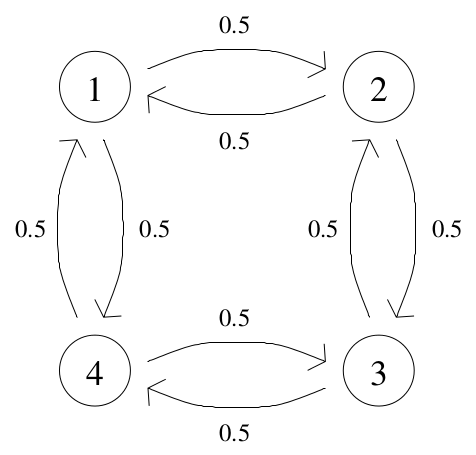
\includegraphics[scale=0.3]{imagens/markovchain}
	\caption{Ilustração de uma simples cadeia de Markov.}
	\label{markovchain}
\end{figure}

\noindent Sendo assim, a matriz estocástica referente ao grafo seria a matriz \eqref{M},

\begin{equation}\label{M}
	D = \begin{pmatrix}
 			0		&	\frac{1}{2}	&	0			&	\frac{1}{2}\\
 		\frac{1}{2}	&	0			&	\frac{1}{2}	&	0\\
 			0		&	\frac{1}{2}	&	0			& 	\frac{1}{2}\\
 		\frac{1}{2}	&	0			&	\frac{1}{2}	&	0
		\end{pmatrix}.
\end{equation} 

\noindent E a simulação em questão seria então dada pela equação \eqref{xBx},

\begin{equation} \label{xBx}
	x(k+1) = D x(k),\qquad k=0,1,2,\ldots.
\end{equation}
%%%%%%%%%%%%%%%%%%%%%%%%%%%%%%%%%%%%%%%%
\chapter{O Algoritmo \textit{PageRank}}%
%%%%%%%%%%%%%%%%%%%%%%%%%%%%%%%%%%%%%%%%

%Proposta do PageRank
O \textit{PageRank} é o principal algoritmo por trás das engrenagens de busca do \textit{Google}, criado em 1998 por Lawrence Page e Sergey Brin \ref{larry} para atribuir pesos a páginas da \textit{Web}. Ele tem como função atribuir um valor numérico para cada elemento em um conjunto de documentos, em que na \textit{Internet} tratariam-se de páginas \textit{Web}. Tendo como principal objetivo a identificação das páginas mais importantes aos usuários da rede, de forma a atribuir valores maiores as páginas mais importantes.

\
\begin{figure}[!htb]
	\centering
	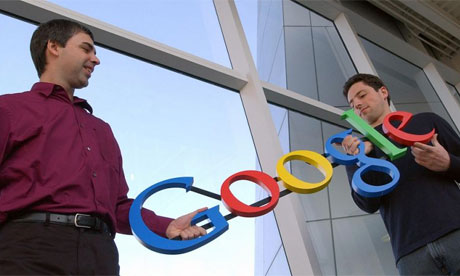
\includegraphics[scale=0.45]{imagens/larry}
	\caption{Lawrence Page e Sergey Brin criadores do \textit{PageRank} e fundadores do Google.}
	\label{larry}
\end{figure}

O \textit{Google} descreve o \textit{PageRank} da seguinte forma: \textit{"O \textit{PageRank} reflete nossa percepção de importância das páginas da \textit{Web} de forma a considerar mais de 500 milhões de variáveis e 2 bilhões de termos. Páginas que são consideradas importantes recebem um maior valor de PageRank, sendo assim, possuem maior possibilidade de aparecerem no topo de um resultado de busca."} 

%O grau de importância das páginas
A respeito da atribuição de importância às páginas, a página mais importante será a mais visitada e a página mais visitada será aquela que está associada a um maior número de \textit{links}. De forma mais precisa o número de visitas de uma página vai estar associado aos \textit{links} de saída que ela possui. Contudo, uma página também pode ser considerada importante por estar próxima a uma página de alto \textit{PageRank}. Algumas páginas famosas e seus \textit{PageRanks} são mostrados na tabela \ref{webrank}.


\vspace{0.3cm}

\
\begin{table}[!htb]
\centering
\begin{tabular}{lllll}
Nome da Página & PageRank\\
google.com & 10\\
ebay.com & 9\\
espn.com & 8\\
ge.com & 7\\
generalmills.com & 6\\
\end{tabular}
\caption{Valores atribuídos a algumas páginas da \textit{Web} pelo Google em 2007.}
\label{webrank}
\end{table}

%Google x PageRank
No trabalho em que foi proposto o \textit{PageRank} em 1998 \cite{brin2012reprint}, é resolvida a questão de como construir um sistema de larga escala para explorar informações adicionais da \textit{Web} de forma a lidar com coleções de páginas e \textit{links} não controlados, onde qualquer usuário da rede pode publicar ou retirar uma página a cada instante. 

Entretanto, o \textit{PageRank} é só uma pequena parte do sistema de buscas do Google. O sistema do buscador parte de uma \textit{query} que é feita na barra de pesquisa do Google \ref{google}, em seguida as palavras que estão contidas nesta \textit{query} são procuradas no conjunto de páginas indexadas pelo buscador. Por fim, o \textit{PageRank} faz o ranqueamento das páginas que possuem a palavra pesquisada.

\
\begin{figure}[!htb]
	\centering
	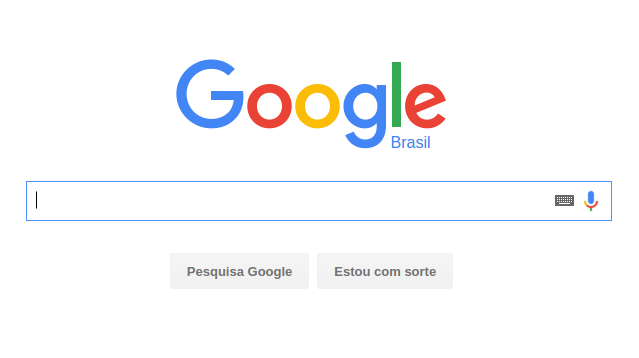
\includegraphics[scale=0.45]{imagens/google}
	\caption{Barra de pesquisa do Google.}
	\label{google}
\end{figure}

Contudo, apesar de toda a complexidade do sistema de busca, o maior problema por trás do buscador é fazer o ranqueamento desse número massivo de páginas. Não por acaso os fundadores escolheram o nome Google para representar a ferramenta de busca que haviam criado, uma vez que a palavra vem de googol, ou $10^{100}$, para representar a massividade da \textit{Web}. 


%%%%%%%%%%%%%%%%%%%%%%%%%%%%%%%%%%
\section{As Ferramentas de Busca}%
%%%%%%%%%%%%%%%%%%%%%%%%%%%%%%%%%%

O histórico de sucesso das ferramentas de busca está associado ao número de páginas indexadas pelos buscadores. Quanto mais páginas indexadas, melhores eram os resultados de busca pois estavam mais adequados ao que procurava o navegador. Desde 1994 tecnologias de busca têm tido que alcançar o crescimento da Web. Como pode-se constatar na tabela \ref{websize}, uma das primeiras ferramentas de busca, a \textit{World Wide Web Worm - WWWW} \cite{mcbryan1994genvl} possuia 110 mil páginas \textit{Web} indexadas. No entanto, em 1997 as melhores ferramentas de busca precisavam ter um índice com cerca de 100 milhões de páginas e em 1998 o Google surge com 518 milhões de páginas indexadas.

\vspace{0.3cm}

\
\begin{table}[!htb]
\centering
\begin{tabular}{lllll}
Ano & Buscador & Nº de Páginas Indexadas\\
1994 & WWWW & 110 mil\\
1997 & AltaVista & 100 milhões\\
1998 & Google & 518 milhões\\
2016 & Google & 4.8 bilhões
\end{tabular}
\caption{Número de páginas indexadas pelos buscadores.}
\label{websize}
\end{table}


%%%%%%%%%%%%%%%%%%%%%%%%%%%%%%%%%%%%%%%%%%
\section{O Problema do \textit{PageRank}}%
%%%%%%%%%%%%%%%%%%%%%%%%%%%%%%%%%%%%%%%%%%

O cálculo do \textit{PageRank} está sujeito a um grande problema, o custo computacional. Através dos dados apresentados na seção anterior, em função da grande dimensão da \textit{Web} pode-se constatar que esse cálculo não é nada trivial. Além do custo computacional, outros problemas surgem ao considerarmos os casos em que um navegador aleatório \cite{avrachenkov2007monte} não segue a estrutura de \textit{Hyperlink}. Assim, são três os principais problemas da simulação do cálculo do \textit{PageRank}: o problema dos \textit{Dark Holes} ou Buracos Negros, o problema da navegação descontínua por páginas não diretamente ligadas e o problema do cálculo do \textit{PageRank} de um conjunto massivo de documentos.

%Apresentação do modelo simples
O \textit{PageRank} pode ser pensado como um modelo que simula o comportamento de um usuário que age de forma aleatória. Considerar que existe um navegador que vai acessando páginas aleatoriamente, de forma a clicar somente em \textit{links} na página em que se encontra, consiste no modelo mais simples de cálculo do \textit{PageRank}. 

%Problema 1 - Buraco negro
Outra importante situação que precisa ser levada em consideração é a possibilidade de um usuário acessar uma página sem links de saída, como por exemplo, um link que o direcione para um documento PDF, como ilustrado na figura \ref{blackhole}. Neste caso o usuário poderia usar o botão de voltar do \textit{Browser} para sair deste tipo de buraco negro na rede, o que simplifica possíveis problemas no cálculo do \textit{PageRank}.  

\
\begin{figure}[!htb]
	\centering
	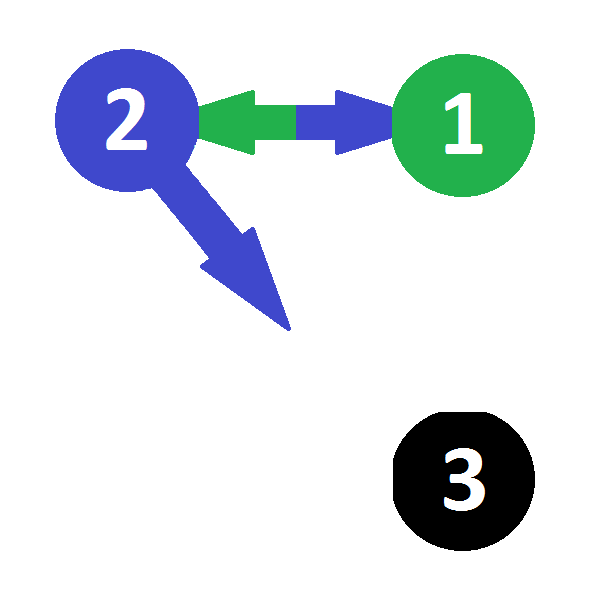
\includegraphics[scale=0.35]{imagens/blackhole1}
	\hspace{0.1cm}
	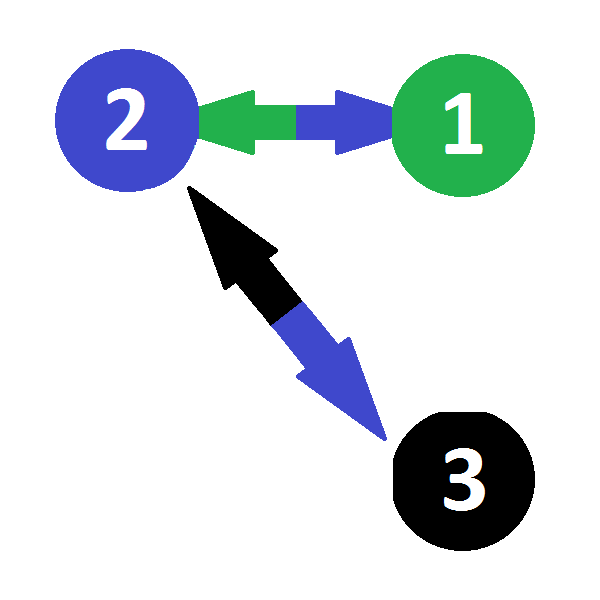
\includegraphics[scale=0.35]{imagens/blackhole2}
	\caption{O buraco negro da \textit{Web}.}
	\label{blackhole}
\end{figure}

%Problema 2 - Teleportation Model
Um outro problema surge ao considerar-se que o usuário pode saltar de uma página para outra sem seguir a estrutura de \textit{links}, por ficar entediado, ou por um outro motivo qualquer. Um exemplo de como isso poderia ocorrer, é o caso do usuário estar na página do Laboratório Nacional de Computação Científica - LNCC e seguindo a estrutura de \textit{Hyperlink}, clicar em um \textit{link} que o leve à página do governo federal. No entanto, o usuário de repente altera o \textit{Uniform Resource Locator - URL} e vai para um \textit{site} de notícias que não está diretamente ligado aos outros dois \textit{sites}. Este exemplo é ilustrado na figura \ref{tele}.

\
\begin{figure}[!htb]
	\centering
	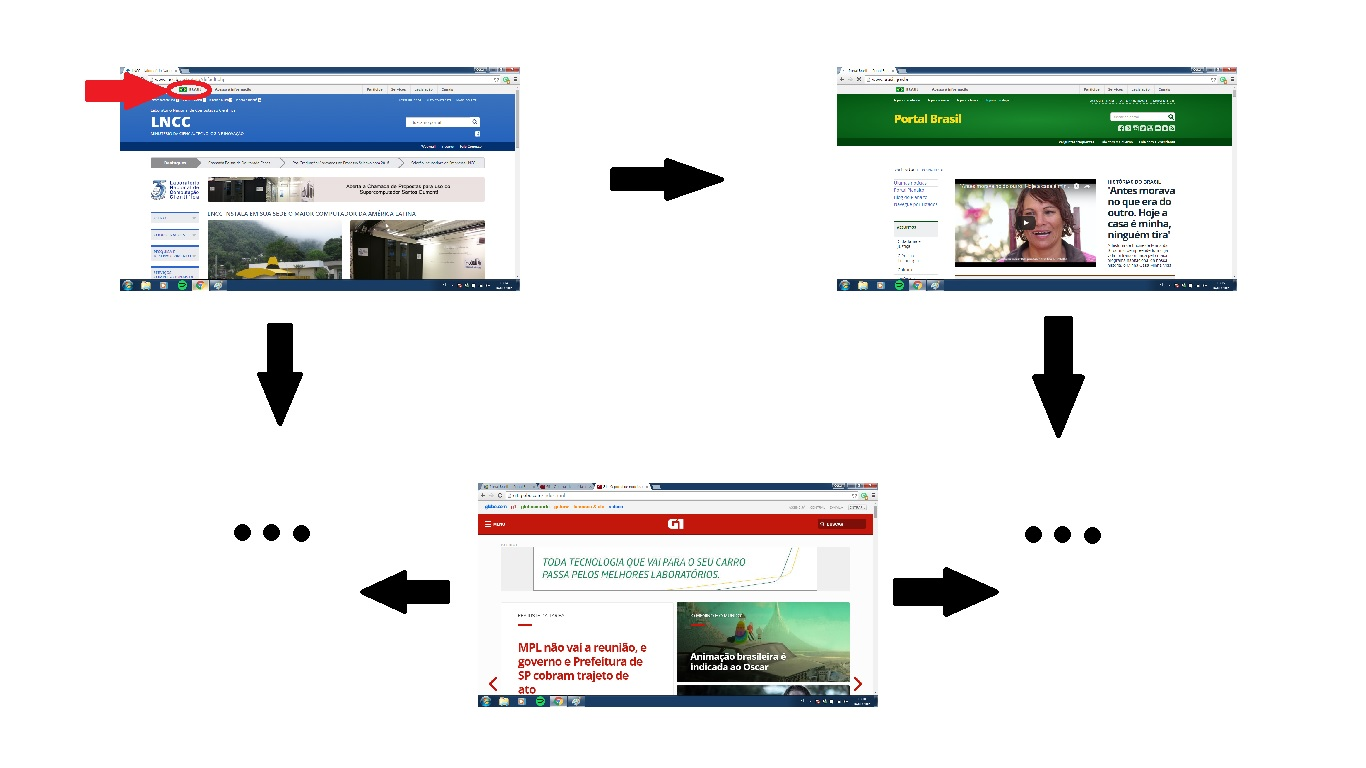
\includegraphics[scale=0.3]{imagens/tele}
	\caption{Navegação entre páginas indiretamente conectadas.}
	\label{tele}
\end{figure}

\noindent Este problema foi apontado pela primeira vez no artigo que deu origem ao Google em 1998 \cite{brin2012reprint}, e foi recentemente apelidado em \cite{ishii2014pagerank} de \textit{Teleportation Model}.

%Problema 3 - A massividade da Web
A massividade da \textit{Web} é uma das principais questões por trás do cálculo do \textit{PageRank}, considerando que a dimensão da \textit{Web} pode tornar o ranqueamento de páginas impossível. No entanto, a solução para este problema é o uso de algoritmos distribuídos, sobre os quais a cada ano novas publicações são feitas \cite{lei2015distributed}. Neste contexto, a fim de melhorar a performance do processamento, o cálculo a partir do modelo distribuído é realizado com a ajuda de vários conputadores num \textit{cluster}, como o da figura \ref{cluster}. Sendo assim, os recursos computacionais já necessários para abrigar a \textit{Web} também seriam usados para o cálculo de \textit{PageRank}.    

\
\begin{figure}[!htb]
	\centering
	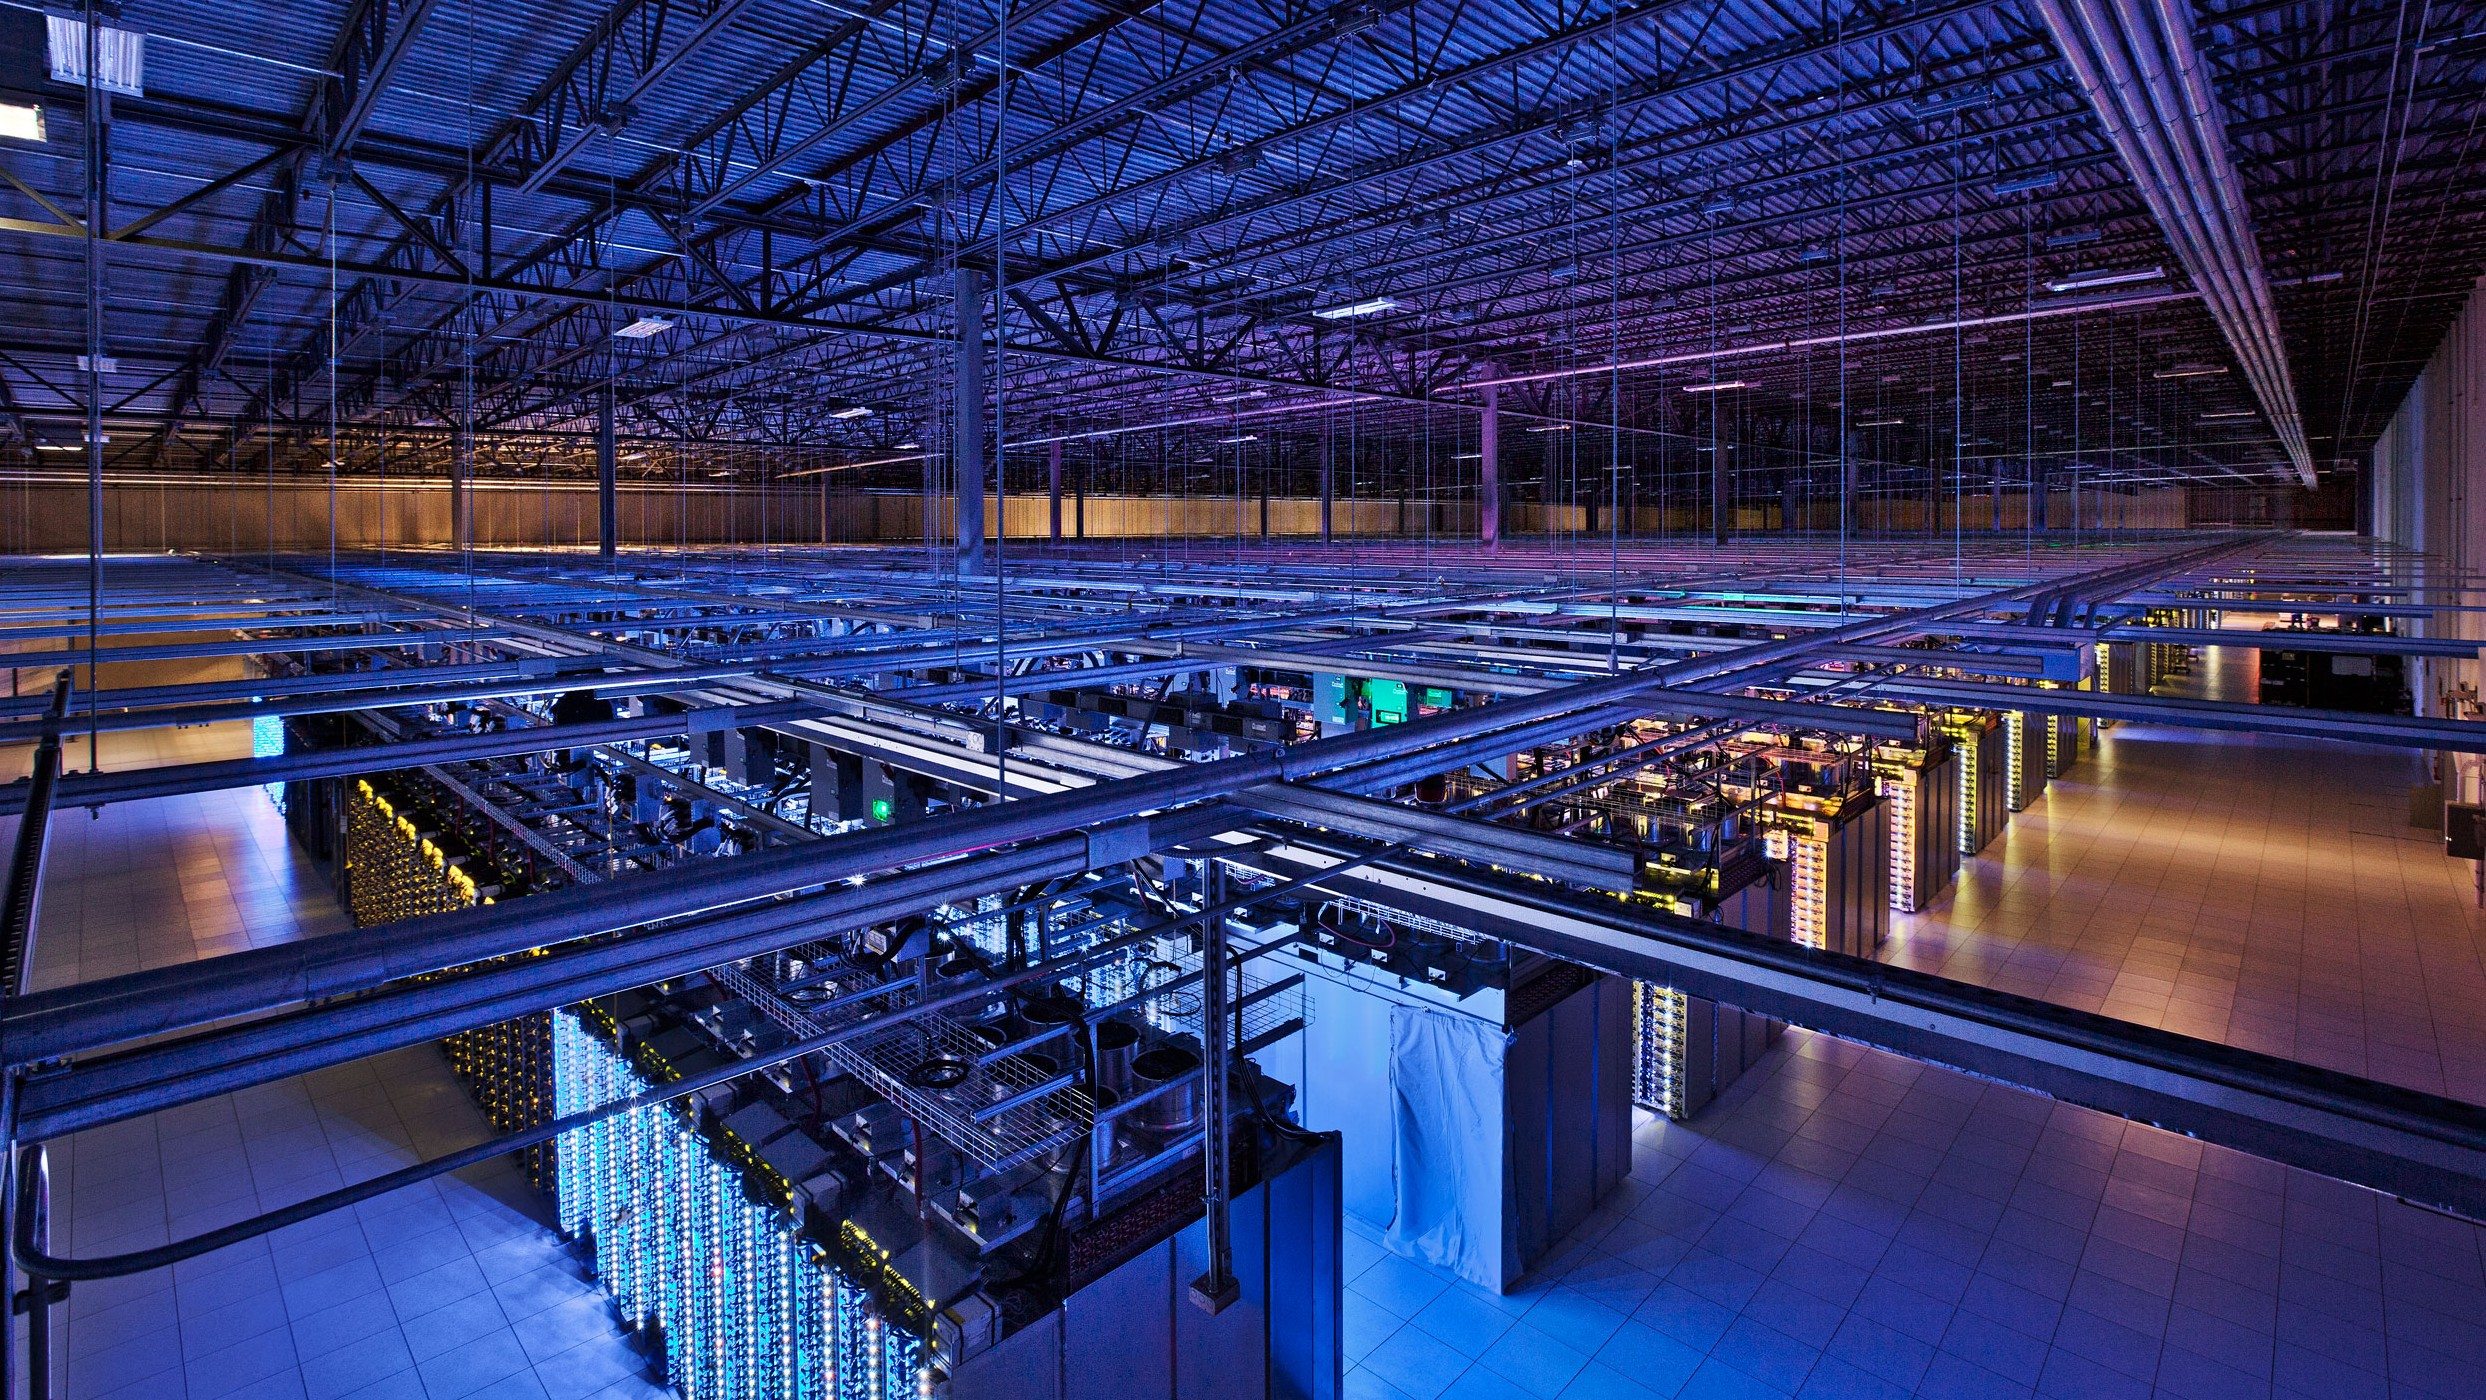
\includegraphics[scale=0.1]{imagens/cluster}
	\caption{Cluster do Google.}
	\label{cluster}
\end{figure}
%%%%%%%%%%%%%%%%%%%%%%%%%%%%%%%%
\chapter{Definição dos Modelos}%
%%%%%%%%%%%%%%%%%%%%%%%%%%%%%%%%

O cálculo do \textit{PageRank} possui desde um modelo mais simples, até outras adaptações deste modelo devido aos problemas descritos na seção anterior. A estimação do \textit{PageRank} é feita por uma equação de diferença, a qual possui uma matriz de transição do tipo estocástica. Na primeira seção deste capítulo é demostrada a construção dessa matriz. Na sequência são apresentados o \textit{Power Method}, modelo mais simples do cálculo do \textit{PageRank}, o \textit{Teleportation Model}, modelo que trata da navegação descontínua e o modelo por trás dos algoritmos distribuídos.   


%%%%%%%%%%%%%%%%%%%%%%%%%%%%%%%%%%%%%%
\section{A Matriz \textit{Hyperlink}}%
%%%%%%%%%%%%%%%%%%%%%%%%%%%%%%%%%%%%%%

A construção da matriz \textit{hyperlink} é feita com base na estrutura da \textit{Web}, ou ainda do grafo que a representa. Assim, considerando que o grafo da figura \ref{grafo} representa um conjunto de páginas interligadas, seus elementos são definidos da seguinte forma: 

\
\begin{figure}[!htb]
	\centering
	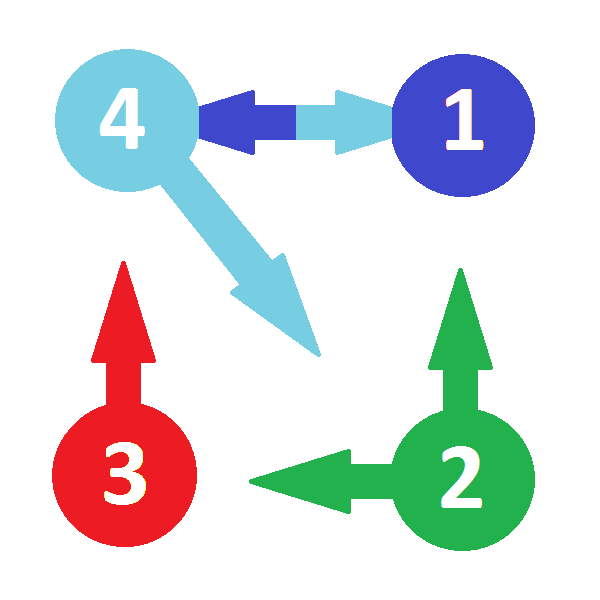
\includegraphics[scale=0.4]{imagens/grafo}
	\caption{Grafo representando \textit{links} entre páginas \textit{Web}.}
	\label{grafo}
\end{figure}

\begin{itemize}
\item $n$: como os n\'os, que representam as p\'aginas,

\vspace{0.1cm}
	
\item $\mathcal{E}$: como as arestas, que representam os \textit{links} entre as páginas.
\end{itemize}

Para representar o \textit{link} entre duas páginas específicas usa-se $i$ e $j$, de forma que o $i$ esteja associado à página de saída e $j$ com a de entrada. Considerando então o caso de um v\'ertice $i$ estar conectado a um $j$, tem-se $(i,j) \in \mathcal{E}$.

A matriz de transição que é construída a partir do grafo tem a seguinte propriedade para cada um de seus elementos:

\begin{equation}\label{a}
a_{ij} = \begin{cases}
\dfrac{1}{n_i}, & \text{caso}\, (i,j)\in \mathcal{E},\\
0, & \text{caso contr\'ario}.
\end{cases}
\end{equation}	

Cada elemento $a_{ij}$ é formado a partir das relações entre os nós do grafo. Para o nó $1$ por exemplo, constata-se que ele só possui relações com o nó $4$, por tanto, para um navegador que encontra-se em $1$ tem-se $100\%$, de certeza de que seu próximo passo será para $4$. Já no caso do nó $2$ pode-se observar que o navegador pode ir para $1$ ou $3$, ou seja, ele tem $50\%$ de chance de ir para cada um desses dois nós.

\begin{equation}\label{A}
A = \begin{pmatrix}
 0 & 1/2 & 0 & 1/2 \\
 0 &  0  & 0 & 1/2 \\
 0 & 1/2 & 0 &  0  \\
 1 &  0  & 1 &  0
\end{pmatrix}
\end{equation}

E assim constroi-se a matriz de transição \eqref{A} de forma que todas as suas colunas respeitem a propriedade:

\begin{equation}\label{n}
\sum^{n}_{i=1} x_{i} = 1.
\end{equation}

Vale ressaltar que partindo de qualquer nó, todos os outros nós ligados a este possuem a mesma probabilidade de serem acessados. Ou seja, em uma página um \textit{link} ou outro não terão maior probabilidade de serem acessados por chamarem mais atenção, ou por qualquer outro motivo.

Sendo assim, o grafo, ou o conjunto de páginas, trata-se de uma cadeia de Markov com espaço de estados de dimensão $n$. Onde a estimação de uma posição seguinte apenas depende da atual.

%, seguindo a propriedade de Markov \ref{p}.

%\begin{equation}\label{p}
%P \bigl( \theta(k+1) = j \mid  \theta(k) = i_k, \theta(k-1) = i_{k-1}, \ldots, \theta(0) = i_0\bigr) = P %\bigl( \theta(k+1) = j \mid  \theta(k) = i_k\bigr).
%\end{equation}


%%%%%%%%%%%%%%%%%%%%%%%%%%%%%%%%%%
\section{O \textit{Power Method}}%
%%%%%%%%%%%%%%%%%%%%%%%%%%%%%%%%%%

Este é o modelo mais simples para a estimação do \textit{PageRank}. Esta abordagem constitui-se de uma equação de diferença, a qual possui uma matriz de transição coluna estocástica e um vetor estocástico. O vetor estocástico é formado pelos valores das variáveis aleatórias da cadeia de Markov, ou seja os valores das páginas. O valor de \textit{PageRank} de um conjunto de $n$ páginas da \textit{Web} é definido como o vetor $x \in \mathbb{R}^{n \times 1}$ que satisfaz as seguintes equações:

\begin{equation}	
x = Ax, \quad x\geq0, \quad \sum^{n}_{i=1} x_{i} = 1, 
\end{equation}

\noindent onde $A \in \mathbb{R}^{n \times n}$ é a transposta da matriz de transição da cadeia de Markov.

Assim, o método usual para obtenção do \textit{PageRank} é o chamado \textit{Power Method} \cite{ishii2014pagerank}, que alcança o \textit{PageRank} através da seguinte iteração:

\begin{equation}
x(k+1) = Ax(k), \quad k\geq0, \quad \text{com} \quad x(0) = x_0,
\end{equation}

\noindent onde $x_0 \in \mathbb{R}^{n \times 1}$ é uma condição inicial positiva de soma igual a um.


%%%%%%%%%%%%%%%%%%%%%%%%%%%%%%%%%%%%%%%%%%%%%%%%%%%%%%%%%%%%%%
\subsection{Questões de Convergência do \textit{Power Method}}%
%%%%%%%%%%%%%%%%%%%%%%%%%%%%%%%%%%%%%%%%%%%%%%%%%%%%%%%%%%%%%%

Após um número considerável de iterações e em um número considerável de casos, o \textit{Power Method} atinge a distribuição limite com os valores de \textit{PageRank} de cada página. Além disso, independente da condição inicial, ao final das iterações os valores de \textit{PageRank} tendem a ser os mesmos.

Isso ocorre devido a matriz de transição ser irredutível, o que reflete no navegador aleatório sempre conseguir chegar a uma certa página partindo de uma outra qualquer, mesmo que essas duas páginas não estejam diretamente conectadas. Observando o grafo da figura \ref{grafo}, pode-se observar que não existe um \textit{link} direto entre $1$ e $3$, para chegar-se em $3$ a partir de $1$ o usuário teria de ir de $1$ para $4$, de $4$ para $2$ e de $2$ para $3$.

No caso de uma página apenas possuir \textit{links} de entrada, como por exemplo, ao acessar-se um documento PDF, o problema é contornado ao admitir-se que o usuário poderia usar o botão de volta do \textit{Browser}, criando um \textit{link} de saída da página. Assim, a matriz mantem-se irredutível, garantindo que para a maioria das condições iniciais os valores de \textit{PageRank} sejam os mesmos ao atingir-se a distribuição limite. No entanto, existem alguns casos em que não há garantia de convergência, e por tanto o modelo do \textit{Power Method} tem de sofrer algumas alterações. 


%%%%%%%%%%%%%%%%%%%%%%%%%%%%%%%%%%%%%%%%%
\section{O \textit{Teleportation Model}}%
%%%%%%%%%%%%%%%%%%%%%%%%%%%%%%%%%%%%%%%%%

O valor de \textit{PageRank} é estimado após inúmeras iterações entre o vetor de valores das páginas e a matriz de transição estocástica. No entanto mesmo observando os valores das páginas em um grande horizonte de tempo, existem casos em que eles não convergem. O modelo do \textit{Power Method} é atraente pela sua simplicidade, entretanto alguns problemas fazem com que ele não ofereça uma garantia de convergência. O maior desses problemas é devido a possibilidade do usuário fazer uma navegação descontínua no grafo, em que ele saltaria de uma página para outra, de forma a não seguir a estrutura de \textit{links} da rede. Todavia, existe um modelo para resolver o problema da navegação com saltos, modelo este conhecido como \textit{Teleportation Model}. 

O \textit{Teleportation Model} é uma estratégia reconhecida para que, através de uma pequena modificação na matriz $A$, o método convirja globalmente para o PageRank. Essa modificação na matriz $A$ é representada como uma combinação convexa de duas matrizes, em que a matriz de transição agora passa a ser $M$, dada por:

\begin{equation}
M = (1-m)A + \frac{m}{n}{\bf11}^T,
\end{equation}

\noindent onde $M \in \mathbb{R}^{n \times n}$, $m \in (0,1)$ e $\textbf{1} \in \mathbb{R}^{N \times 1}$. Em que $\textbf{11}^T$ é uma matriz preenchida de 1's, resultante do produto entre um vetor de 1's $\textbf{1}$ e um vetor de 1's transposto $\textbf{1}^T$. Vale lembrar também que $n$ é o número de nós do grafo, ou número de páginas, e que $A$ continua sendo a mesma matriz de transição, apenas é substituida por $M$ na equação apresentada no \textit{Power Method}.


%%%%%%%%%%%%%%%%%%%%%%%%%%%%%%%%%%%%%%%%%%%%%%%%%
\section{O Modelo dos Algoritmos Distribu\'idos}%
%%%%%%%%%%%%%%%%%%%%%%%%%%%%%%%%%%%%%%%%%%%%%%%%%

Por fim, um último problema é considerado antes de serem feitas as simulações, a massividade da \textit{Web}. O fato da \textit{internet} ter um grande número de páginas, faz com que o tempo necessário para o cálculo e ranqueamento das páginas seja extremamente grande. A fim de tornar o cálculo do \textit{PageRank} menos custoso, e melhor explorar os recursos computacionais dos servidores disponíveis na web, uma alternativa é o emprego de algoritmos distribuídos. A agregação de tais experimentos aleatórios faz então com que o \textit{power method} se torne um sistema linear com saltos Markovianos do seguinte tipo:

\begin{equation}
	x(k+1) = A_{\theta(k)}x(k), \quad k\geq0, \quad \text{com} \quad x(0) = x_0. 
\end{equation}

Em que a matriz de transição $A$ agora passa a ser várias matrizes \textit{links} distribu\'idas $A_i \in \mathbb{R}^{n \times n}, \: i = 1,2, ..., n$. Sendo cada uma das matrizes distribuídas definidas da seguinte forma: 

\begin{itemize}
\item a i-ésima coluna de $A_i$ coincide com a i-ésima coluna de $A$,
\item a j-ésima entrada diagonal de $A_i$ é igual a um,
\item para $j = 1, ..., n, \: j \neq i$, todas as outras entradas $a_{ij}$ são iguais a zero.
\end{itemize}

A ideia agora é de que cada página fará o seu cálculo de \textit{PageRank}, por isso são criadas as matrizes  distribuídas. Com relação a construção das matrizes, pode-se observar que elas seguem a seguinte ideia. As colunas das matrizes são formadas pelas relações de saída de cada um dos nós, ao mesmo tempo que cada matriz \textit{link} distribuída está associada a um nó do grafo da figura \ref{grafo}. Assim a coluna $1$ de $A$ \eqref{A} é copiada para a primeira coluna de $A_1$ \eqref{A12}, o restante da diagonal pricipal é preenchida com 1's e o restante dos elementos é zero. O mesmo se repete para as outras matrizes distribuídas.

\begin{equation}\label{A12}
A_1 = \begin{pmatrix}
 0 &  0  & 0 &  0 \\
 0 &  1  & 0 &  0 \\
 0 &  0  & 1 &  0  \\
 1 &  0  & 0 &  1
\end{pmatrix}
%
\hspace{0.5cm}
%
A_2 = \begin{pmatrix}
 1 & 1/2 & 0 &  0 \\
 0 &  0  & 0 &  0 \\
 0 & 1/2 & 1 &  0  \\
 0 &  0  & 0 &  1
\end{pmatrix}
\end{equation}

\vspace{0.1cm}

\begin{equation}\label{A34}
A_3 = \begin{pmatrix}
 1 &  0  & 0 &  0 \\
 0 &  1  & 0 &  0 \\
 0 &  0  & 0 &  0  \\
 0 &  0  & 1 &  1
\end{pmatrix}
%
\hspace{0.5cm}
%
A_4 = \begin{pmatrix}
 1 &  0  & 0 & 1/2 \\
 0 &  1  & 0 & 1/2 \\
 0 &  0  & 1 &  0  \\
 0 &  0  & 0 &  0
\end{pmatrix}
\end{equation}	

Acoplando agora o modelo das matrizes distribuídas ao modelo do \textit{Teleportation} tem-se \eqref{Ax},

\begin{equation} \label{Ax}
x(k+1) = (1 - \hat{m})A_{\theta(k)}x(k) + \frac{\hat{m}}{N} \textbf{11}^T, \quad k \geq 0, \quad \text{com} \quad x(0) = x_0,
\end{equation}

\noindent onde $\hat{m}$ é definido como: 

\begin{equation}\label{m}
\hat{m} = \frac{2m}{n-m(n-2)},
\end{equation}

\noindent e $m = 0.15$, é um parâmetro que foi obtido através de testes em \cite{zaki2012detection}.    

%%%%%%%%%%%%%%%%%%%%%%%%%%%%%%%%%%%%%%%%%%%%%%%%%%%%%%%%%%%%
\subsection{Questões de Convergência do Modelo Distribuído}%
%%%%%%%%%%%%%%%%%%%%%%%%%%%%%%%%%%%%%%%%%%%%%%%%%%%%%%%%%%%%

De forma similar ao que ocorre no \textit{Power Method}, este método apresenta problemas de convergência, pois as matrizes $A_1$, $A_2$, $A_3$ e $A_4$ não são irredutíveis. Isso ocorre devido a inserção de 1's nas diagonais, o que na prática implicaria no nó $4$ só ter saída e chegada nele mesmo. Dessa forma, usando-se da matriz $A_1$, por exemplo, um navegador aleatório que partisse de $4$, nunca sairia de lá.

Para isso é usada uma média no tempo, em que a cada iteração é feita uma média de todos os estados anteriores. Assim $y(k)$ é a média do conjunto de amostras $x(0),... , x(k)$ definida como \eqref{y}, 

\begin{equation}\label{y}
y(k) = \frac{1}{k+1} \sum_{l=0}^{k} x(l).
\end{equation}

%De tal forma que o algoritmo converge no sentido da média quadrática \eqref{E}, em que quanto maior é o número de iterações $k$, mais o valor se aproxima da distribuição limite, ou seja, do valor de \textit{PageRank}. 

\noindent De tal forma que o algoritmo converge no sentido da média quadrada, ou seja,

\begin{equation}\label{E}
\lim_{k\rightarrow \infty} \mathbb{E} [\parallel y(k)-x^*\parallel^2] = 0.
\end{equation}

\noindent Neste contexto, quanto maior for o número de iterações $k$, mais o valor de $y(k)$ se aproxima da
distribuição limite, o que representa o valor de \textit{PageRank}.

A fim de minimizar custos computacionais, um formato recursivo da média $y(k)$ foi usado nas simulações, que possui o seguinte formato:

\begin{equation}\label{yr}
	y(k+1) = \frac{(k+1)}{(k+2)}y(k) + \frac{1}{(k+2)}x(k+1).
\end{equation}

%Por que essa estratégia diminui o custocomputacional?
A média em seu formato recursivo \eqref{yr} diminui o custo computacional pois a cada nova iteração do vetor $y(k)$ apenas leva-se em conta o seu estado anterior $y(k-1)$. A média em seu formato comum \eqref{y} é estimada a cada nova iteração a partir de todos os outros estados anteriores, o que eleva consideravelmente o custo computacional. A dedução do modelo recursivo da média é apresentado no Apêndice A.
%%%%%%%%%%%%%%%%%%%%%
\chapter{Simulações}%
%%%%%%%%%%%%%%%%%%%%%

Neste capítulo são apresentadas as simulações feitas dos modelos anteriormente apresentados. Na realização das simulações optou-se pelo uso da linguagem MatLab, por ser simples e conveniente em um primeiro momento, em que não seria necessário um grande poder de processamento. O código em Matlab das simulações encontra-se no Apêndice B. O exemplo usado nas simulações é de um conjunto de quatro páginas \textit{Web}, ou seja, um grafo de quatro nós, ou ainda, uma cadeia de Markov com quatro estados. As simulações foram feitas a partir dos modelos descritos anteriormente e a partir do grafo da figura \ref{grafoSimu} com o objetivo de observar algumas considerações feitas na literatura.

\begin{figure}[!htb]
	\centering
	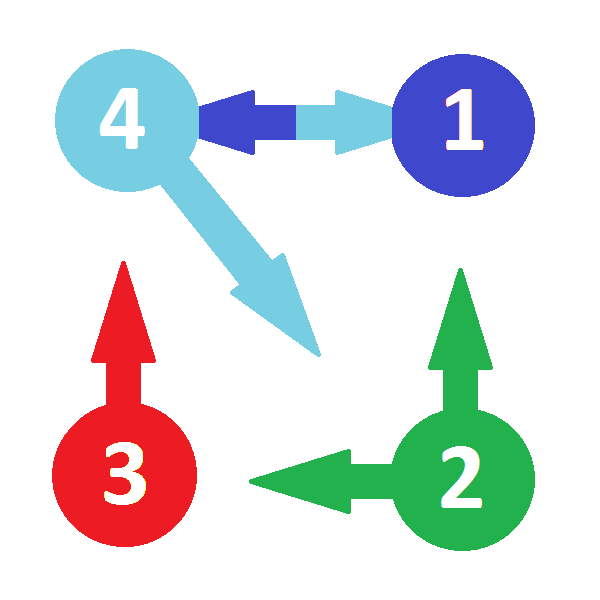
\includegraphics[scale=0.4]{imagens/grafo}
	\caption{Grafo usado nas simulações.}
	\label{grafoSimu}
\end{figure}

\noindent Além disso, todas as simulações foram realizadas com base na seguinte condição inicial:

\begin{equation}\label{x0}
x_0 = \begin{pmatrix}
0\\ 0\\ 0\\ 1
\end{pmatrix}.
\end{equation}

%%%%%%%%%%%%%%%%%%%%%%%%%%%%%%%%%%%%%%%%%%%%%
\section{Simulação do \textit{Power Method}}%
%%%%%%%%%%%%%%%%%%%%%%%%%%%%%%%%%%%%%%%%%%%%%

Na simulação do modelo mais simples do cálculo do \textit{PageRank}, o \textit{Power Method}, observa-se uma rápida convergência para cada um dos valores do vetor de estados. Isso ocorre devido a dimensão do problema usado na simulação. As cores das linhas dos gráficos, que representam os resultados das simulações, seguem o mesmo esquema das cores do grafo na figura \ref{grafoSimu}. Desta forma, as linhas do gráfico estão associadas às páginas da seguinte forma: 

\begin{itemize}
\item página 1: azul escuro,
\item página 2: verde,
\item página 3: vermelho,
\item página 4: azul claro.
\end{itemize}

\
\begin{figure}[!htb]
	\centering
	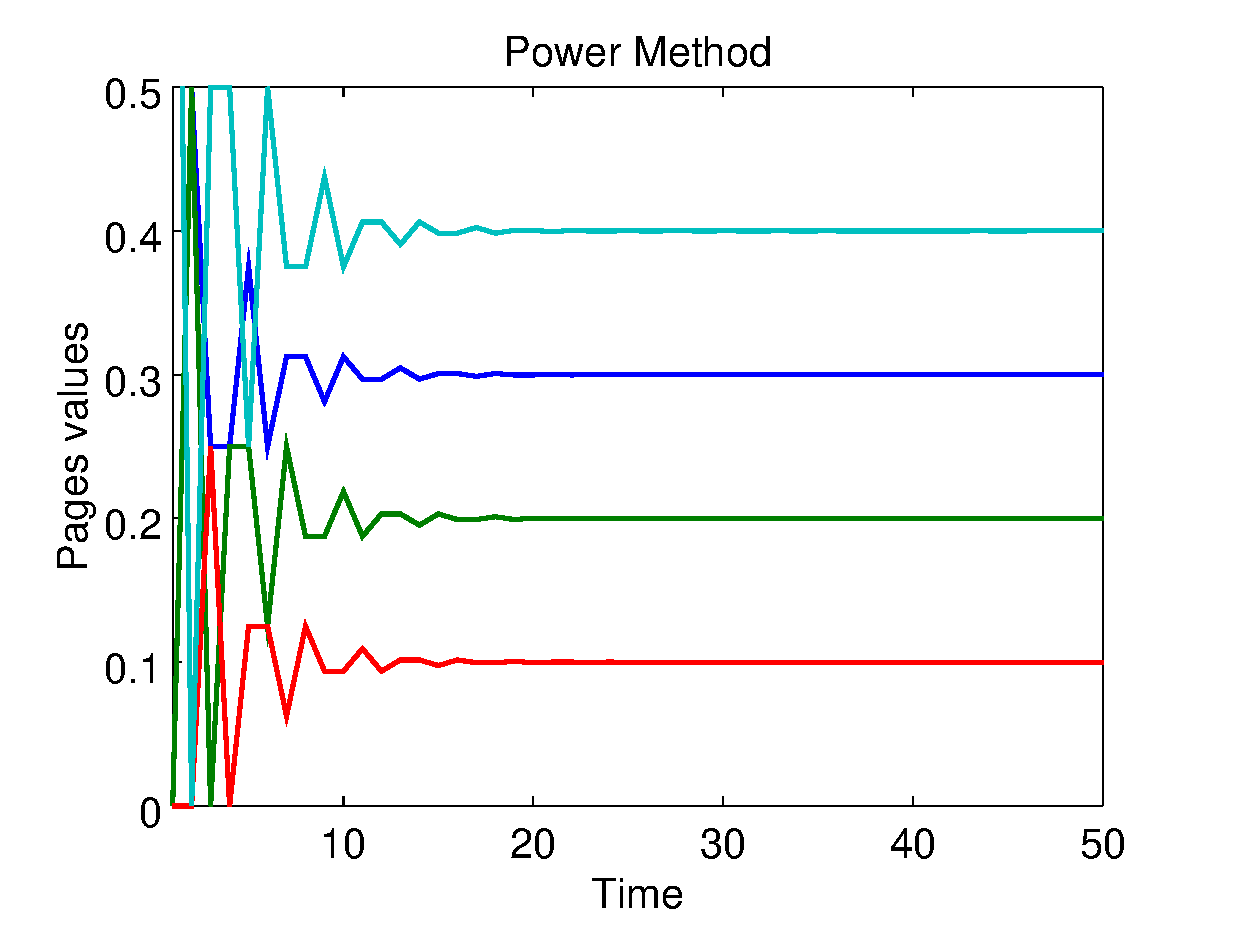
\includegraphics[scale=0.4]{imagens/powermethod}
	\caption{Resultado das simulações do \textit{Power Method}.}
	\label{powermethod}
\end{figure}

Assim pode-se observar que a página de número $4$ foi a que recebeu um maior \textit{PageRank}, dentro deste conjunto de páginas. Ao mesmo que $4$ é a página que está associada a um maior número de links, tanto de entrada quanto de saída, o que define seu alto valor de \textit{PageRank}.

Entretanto, um resultado em primeira vista parece não ser conveniente ao grafo. Ao analisar-se o valor final de $1$ observa-se que ele está na frente da página $2$, e $2$ possui mais \textit{links} de saída que $1$. Fazendo-se uma análise mais cuidadosa nota-se que $1$ possui \textit{links} de entrada e saída para $4$, ou seja por estar ligada a $4$ e por $4$ possuir alto \textit{PageRank}, o número de acessos a $1$ foi maior por estar próximo a uma página supostamente importante.     

%%%%%%%%%%%%%%%%%%%%%%%%%%%%%%%%%%%%%%%%%%%%%%%%%%%%
\section{Simulação do \textit{Teleportation Model}}%
%%%%%%%%%%%%%%%%%%%%%%%%%%%%%%%%%%%%%%%%%%%%%%%%%%%%

Na simulação do \textit{Teleportation Model}, figura \ref{teleportation}, também observa-se uma rápida convergência como nos resultados da simulação do \textit{Power Method}.

\
\begin{figure}[!htb]
	\centering
	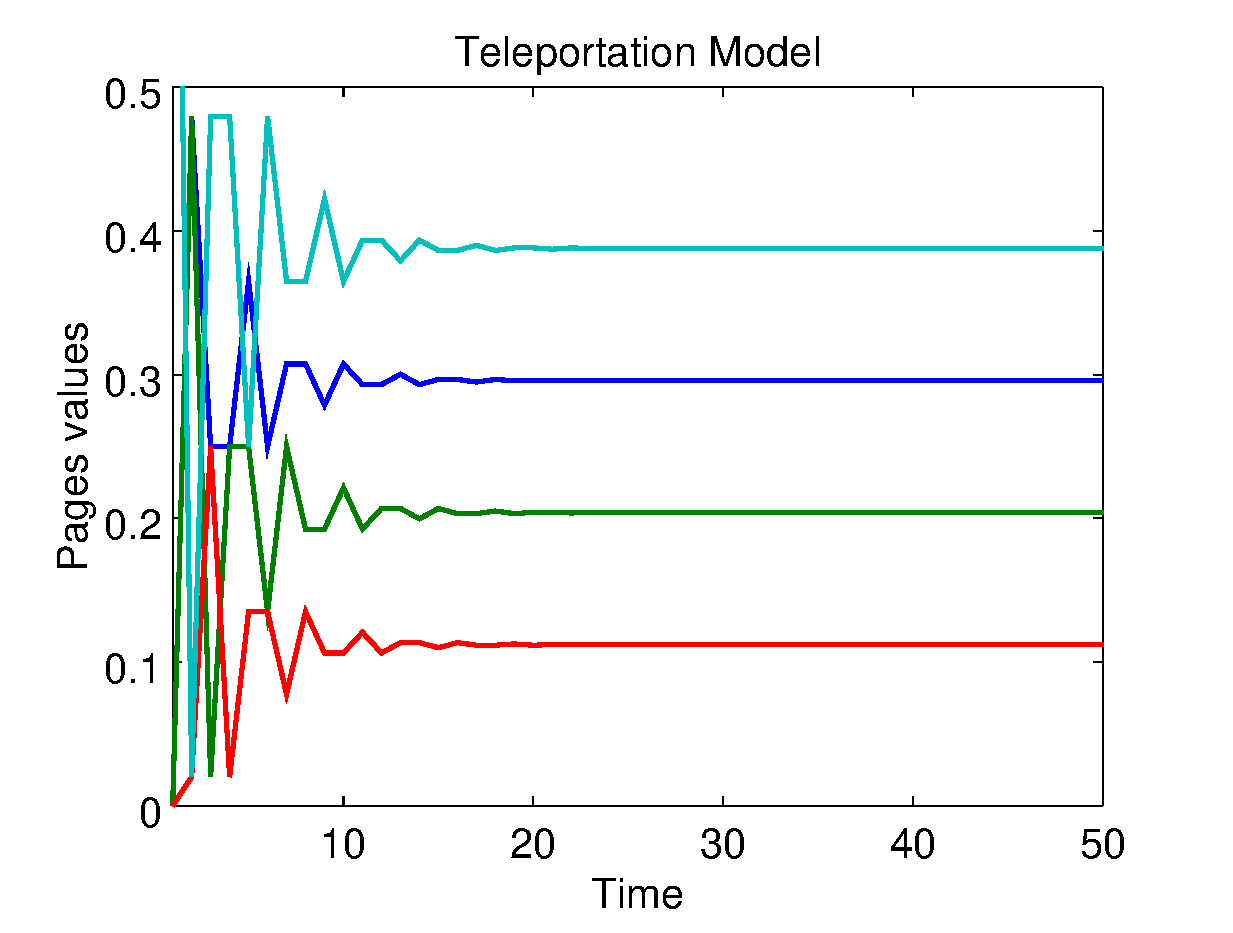
\includegraphics[scale=0.4]{imagens/teleportation}
	\caption{Resultado das simulações do \textit{Teleportation Model}.}
	\label{teleportation}
\end{figure}

Além disso uma grande semelhança é observada entre as duas simulações, como pode-se constatar na figura \ref{powertele}. Tanto a semelhança quanto a rápida convergência se devem ao fato do exemplo simulado não possuir um enorme número de estados $n$ e por ser bem comportado.

\
\begin{figure}[!htb]
	\centering
	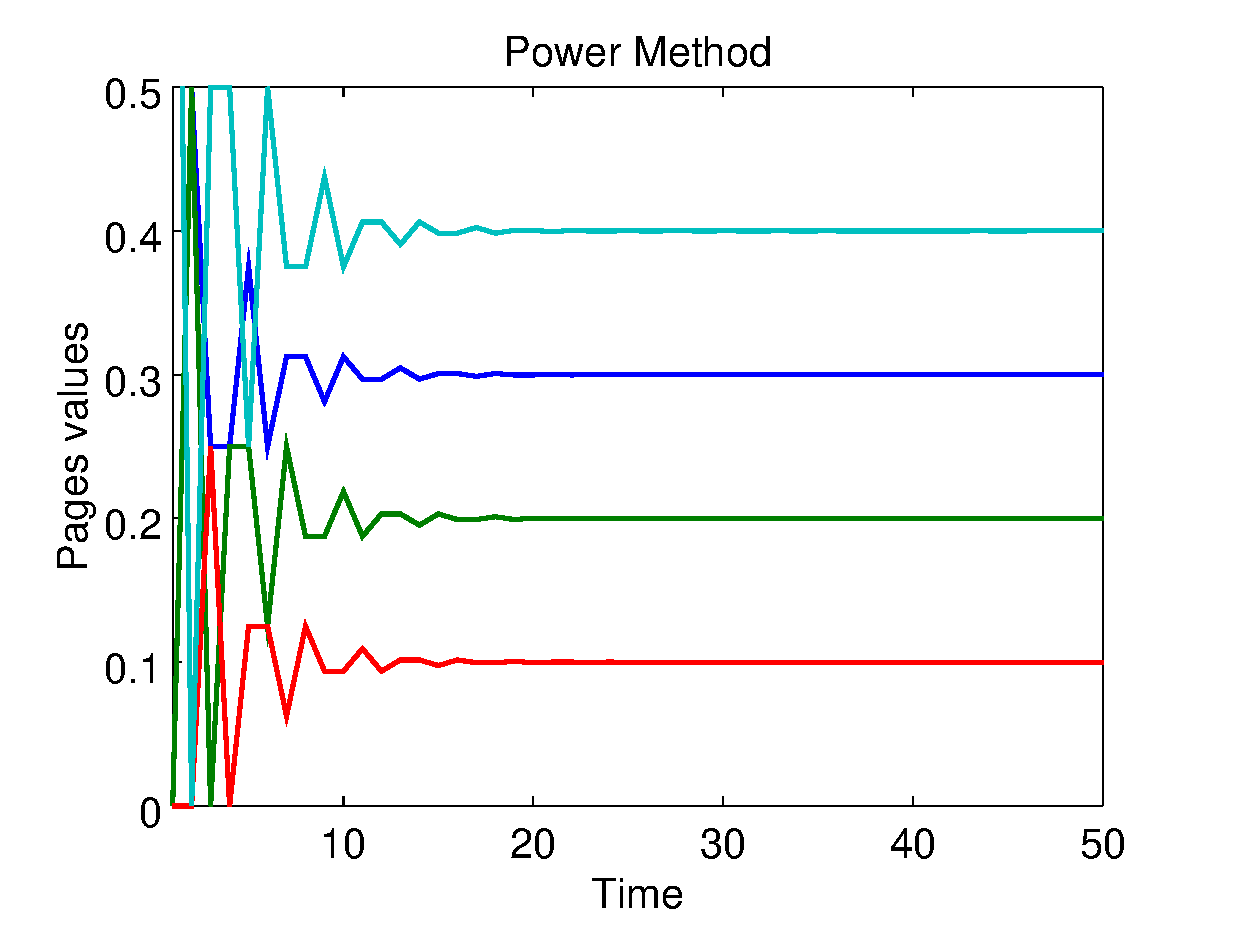
\includegraphics[scale=0.35]{imagens/powermethod}
	\hspace{0.1cm}
	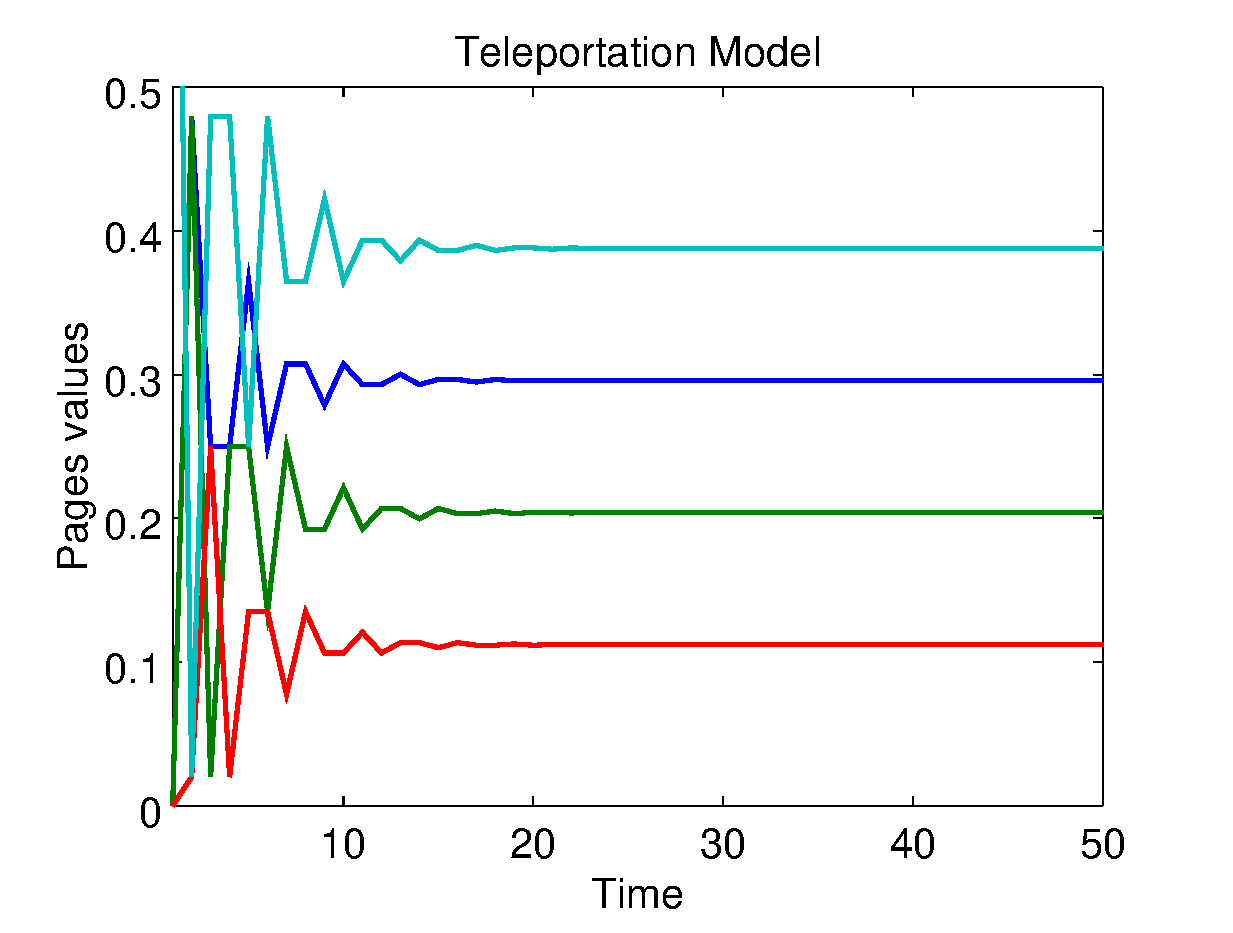
\includegraphics[scale=0.35]{imagens/teleportation}
	\caption{Comparação entre o \textit{Power Method} e o \textit{Teleportation Model}.}
	\label{powertele}
\end{figure}

%%%%%%%%%%%%%%%%%%%%%%%%%%%%%%%%%%%%%%%%%%%
\section{Simulações do Modelo Distribuído}%
%%%%%%%%%%%%%%%%%%%%%%%%%%%%%%%%%%%%%%%%%%%

As simulações do modelo distribuído foram divididas em duas subseções, uma com os resultados do modelo distribuído sem a média no tempo e outra com a média no tempo em sua forma recursiva. É possível observar que os resultados convergem com a média e não convergem sem ela.


%%%%%%%%%%%%%%%%%%%%%%%%%%%%%%%%%%%%%%%%%%%%%%%%%%%%%%%%%%%%%%%%%%%
\subsection{Simulação do \textit{Teleportation Model} Distribuído}%
%%%%%%%%%%%%%%%%%%%%%%%%%%%%%%%%%%%%%%%%%%%%%%%%%%%%%%%%%%%%%%%%%%%

No modelo distribuído sem a média no tempo observa-se uma oscilação dos estados sem que os valores das variáveis aleatórias atinjam a distribuição limite, ou seja, neste modelo sem a média no tempo não foi possível encontrar um valor de \textit{PageRank} mesmo depois de $500$ iterações. Os resultados dessa simulação estão apresentados na figura \ref{teledistributed}.

\
\begin{figure}[!htb]
	\centering
	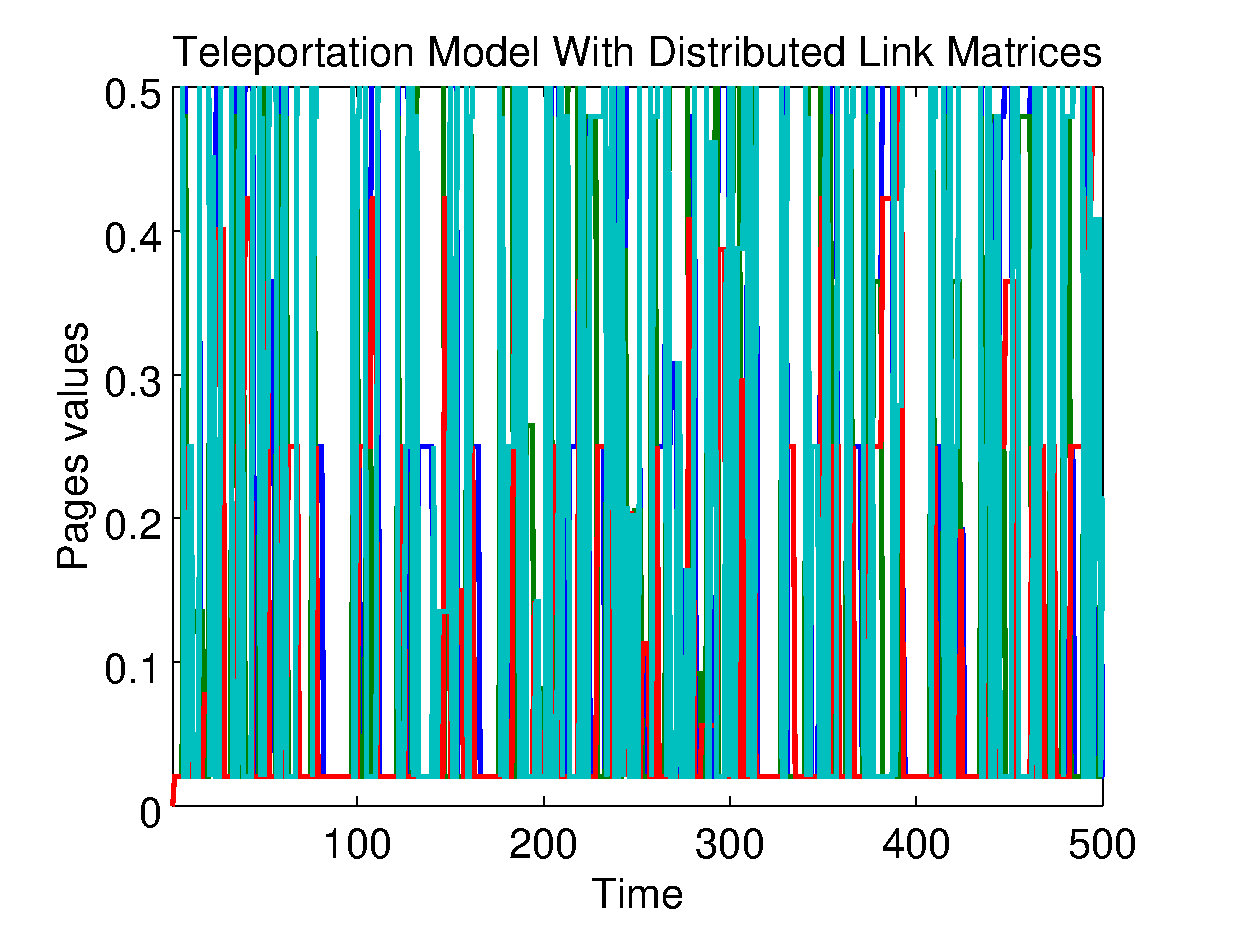
\includegraphics[scale=0.4]{imagens/teledistributed}
	\caption{Resultado das simulações do modelo distribuído.}
	\label{teledistributed}
\end{figure}

A não convergência ocorre devido as matrizes distribuídas possuirem 1's em suas diagonais, o que implicaria, por exemplo, usando-se a matriz $A_1$ como referência, nos nós $2$, $3$ e $4$ só terem saídas para si mesmo, seguindo o esquema apresentado na figura \ref{loop}.

\
\begin{figure}[!htb]
	\centering
	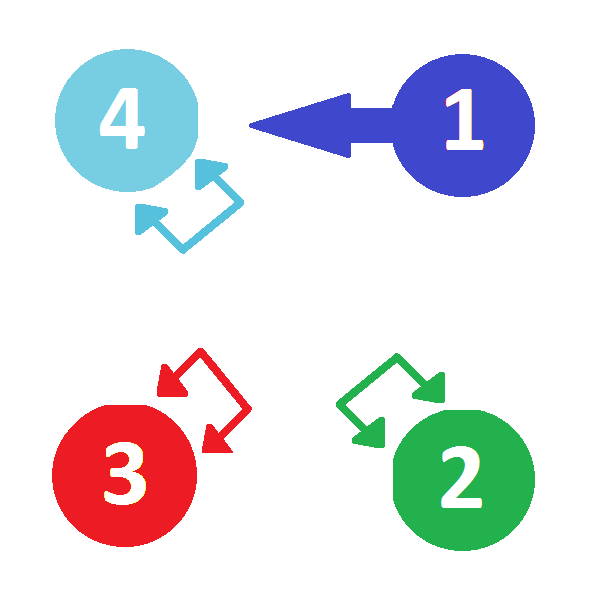
\includegraphics[scale=0.4]{imagens/loop}
	\caption{Abstração dos \textit{links} das páginas 2, 3 e 4 a partir da matriz $A_1$.}
	\label{loop}
\end{figure}

%%%%%%%%%%%%%%%%%%%%%%%%%%%%%%%%%%%%%%%%%%%%%%%%%%%%%%%%%%%%%%%%%%%%%%%%%%%%%%%%%%%%%%%%%%%%%
\subsection{O Modelo Recursivo da Média no Tempo Aplicada a Simulação do Modelo Distribuído}%
%%%%%%%%%%%%%%%%%%%%%%%%%%%%%%%%%%%%%%%%%%%%%%%%%%%%%%%%%%%%%%%%%%%%%%%%%%%%%%%%%%%%%%%%%%%%%

Entretanto, feita a média dos valores do modelo distribuído os resultados convergem, conforme é mostrado na figura \ref{timerecursive}. Mas ainda assim é possível observar algumas oscilações no gráfico, esta simulação também foi feita ao longo de $500$ iterações.

\
\begin{figure}[!htb]
	\centering
	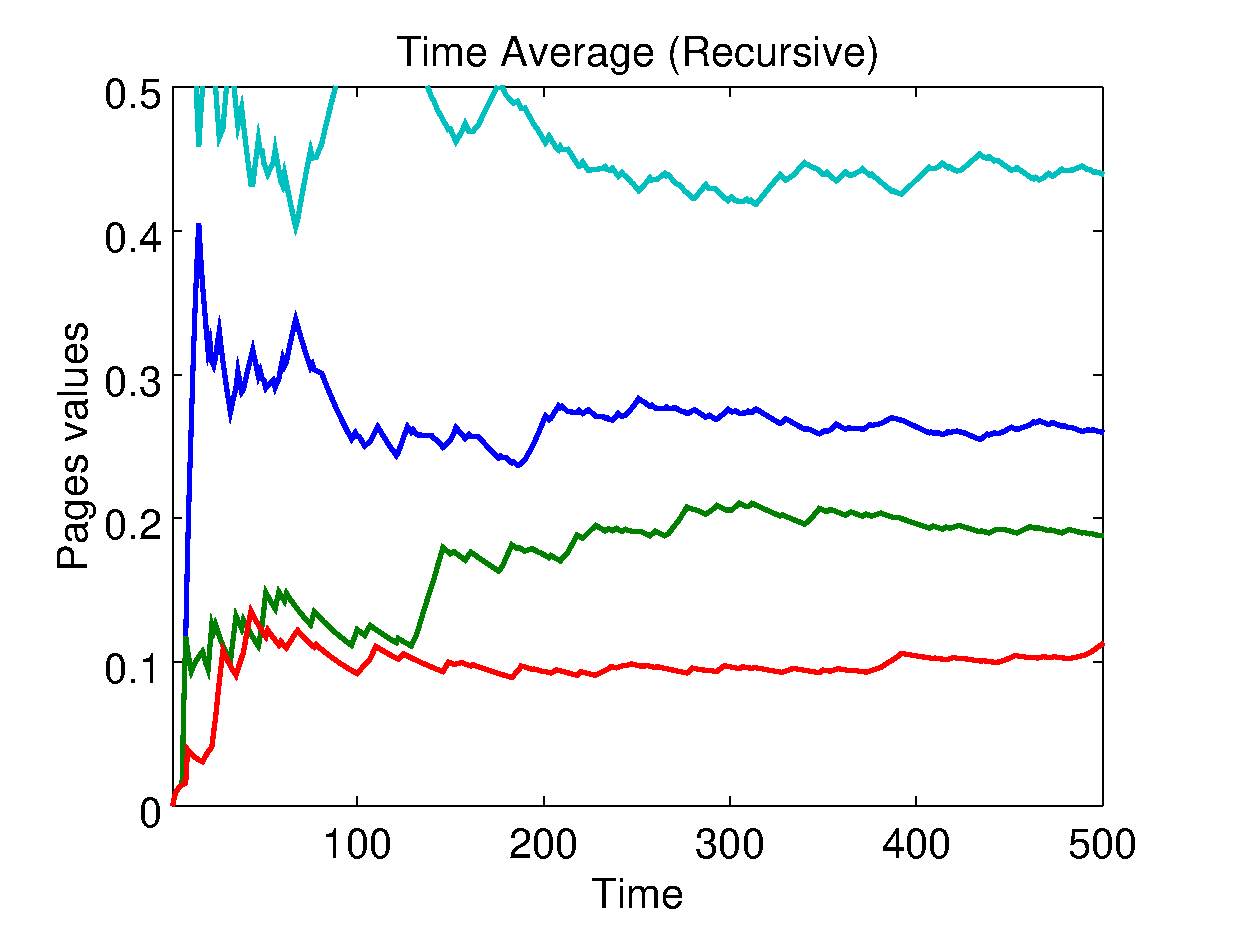
\includegraphics[scale=0.4]{imagens/timerecursive}
	\caption{Resultado das simulações do modelo distribuído com a média no tempo.}
	\label{timerecursive}
\end{figure}

Além disso, observa-se que na distribuição limite são atingidos valores bem próximos aos anteriormente encontrados para cada um dos estados no modelo do \textit{Power Method}, o que pode ser constatado a partir da figura \ref{powertime}.

\
\begin{figure}[!htb]
	\centering
	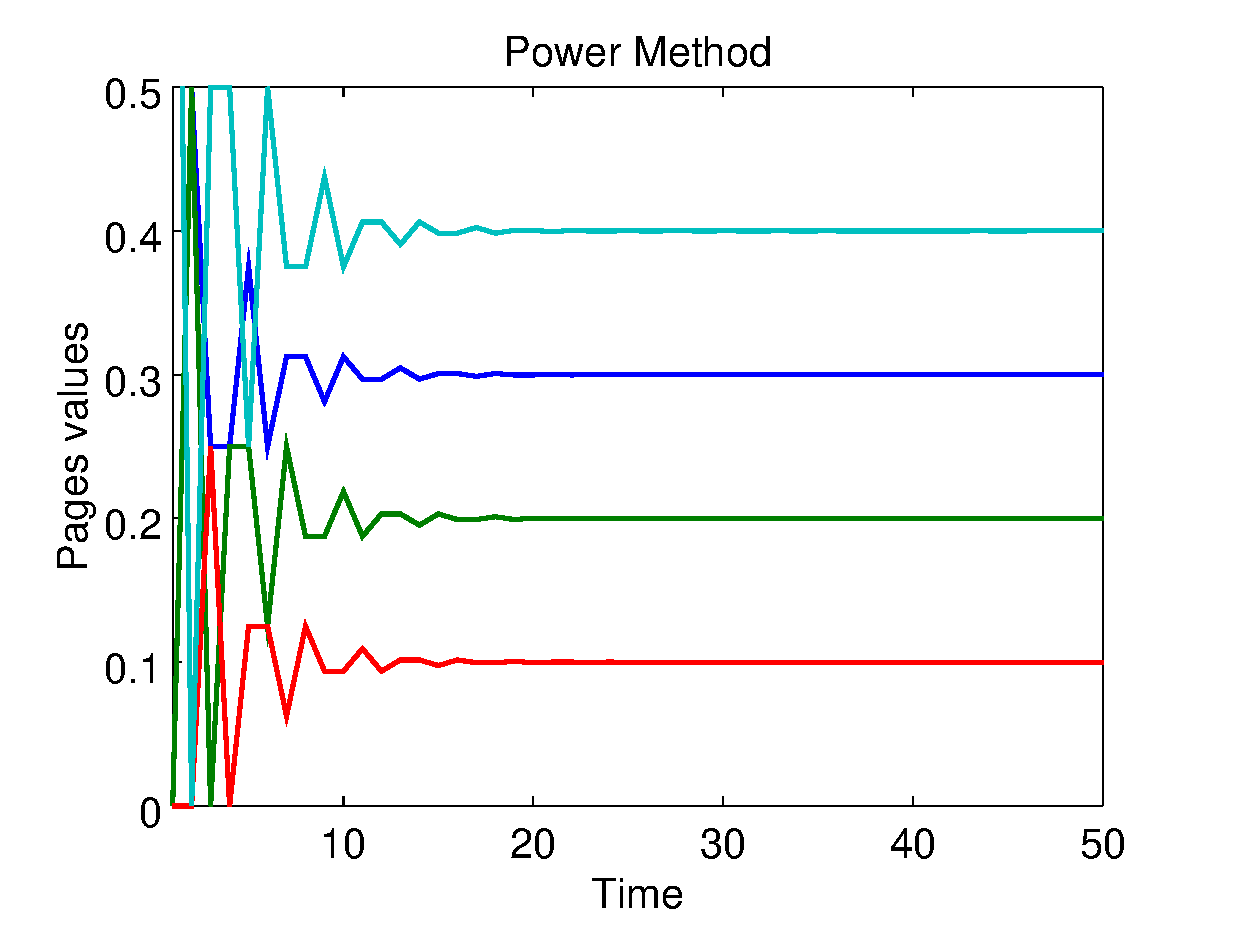
\includegraphics[scale=0.35]{imagens/powermethod}
	\hspace{0.1cm}
	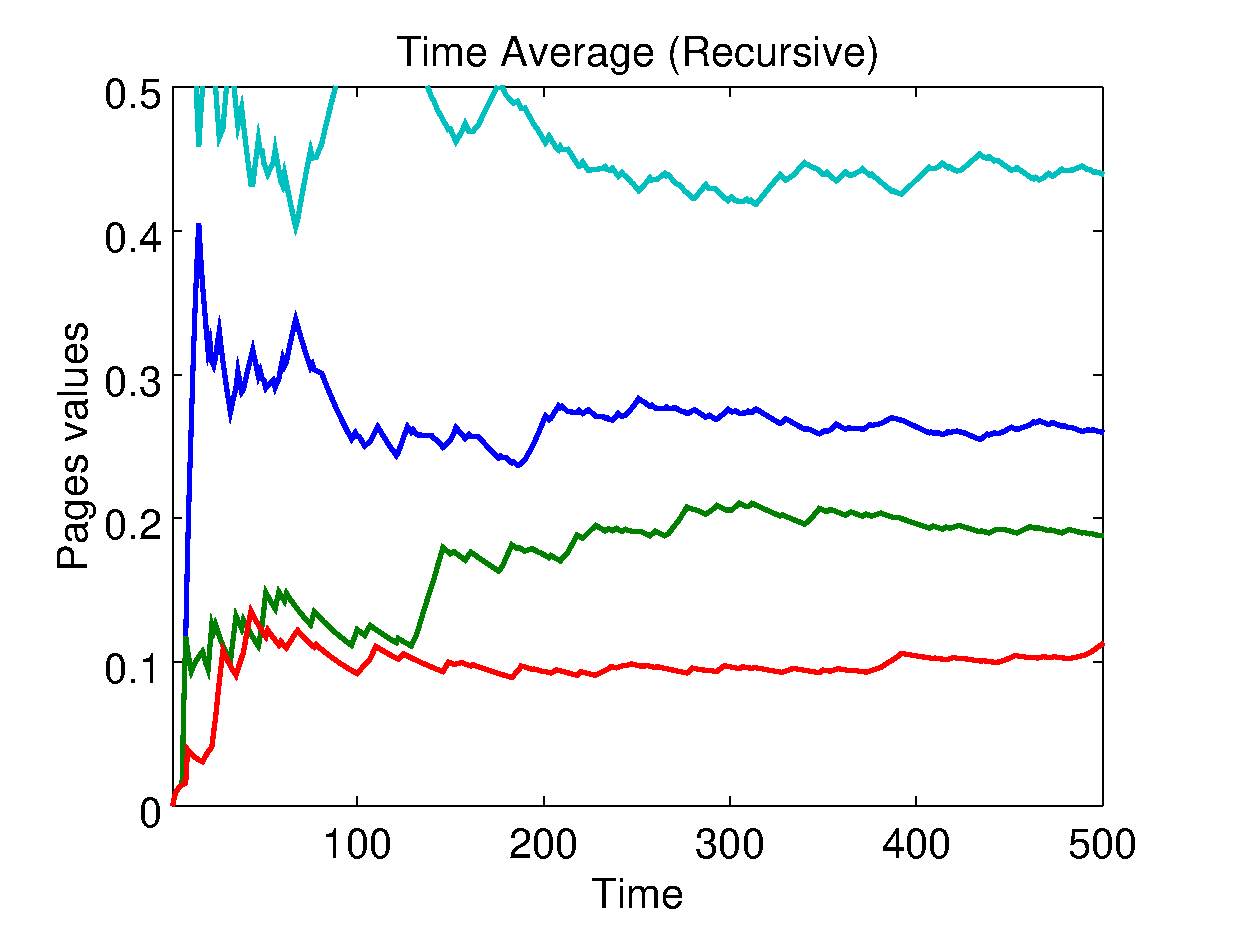
\includegraphics[scale=0.35]{imagens/timerecursive}
	\caption{Comparação entre o \textit{Power Method} e a média no tempo do modelo distribuído.}
	\label{powertime}
\end{figure}


%%%%%%%%%%%%%%%%%%%%%%%%%%%%%%%%%%%%%%%%%%%%%%%%%%%%%%%%%%%%%%%%%%%%%%%%%%%%%%%%%
\section{Método de \textit{Monte Carlo} Aplicado após Modelo Recursivo da Média}%
%%%%%%%%%%%%%%%%%%%%%%%%%%%%%%%%%%%%%%%%%%%%%%%%%%%%%%%%%%%%%%%%%%%%%%%%%%%%%%%%%

Por fim, foi feita uma simulação usando método de Monte Carlo \cite{avrachenkov2007monte}, no qual para cada uma das $500$ iterações que podem ser vistas no gráfico foram feitas mais $500$ iterações antes dos resultados serem plotados de forma a fazer uma média com os valores obtidos depois da média no tempo. Os resultados desta simulação encontram-se na figura \ref{montecarlo}.

\
\begin{figure}[!htb]
	\centering
	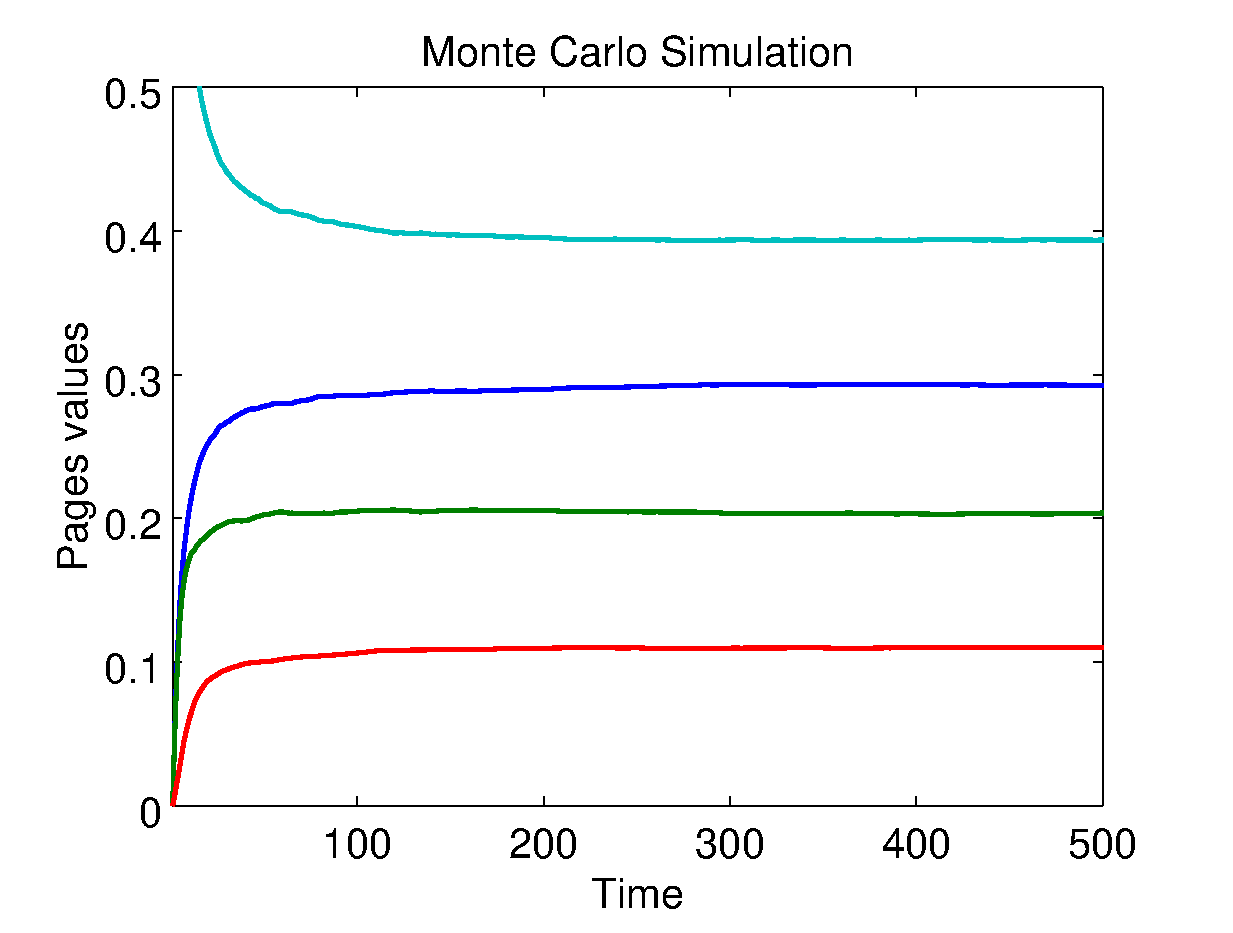
\includegraphics[scale=0.4]{imagens/montecarlo}
	\caption{Resultado das simulações com o método de Monte Carlo.}
	\label{montecarlo}
\end{figure}

Comparando a simulação em que usou-se do método de Monte Carlo com a simulação da média no tempo, observa-se que o gráfico do método de Monte Carlo possui uma curva mais suavizada, o que pode ser constatado nos resultados apresentados na figura \ref{montecarlo}. Além disso a evolução dos valores está mais bem definida, principalmente quando comparados ao valor final da distribuição limite.

\
\begin{figure}[!htb]
	\centering
	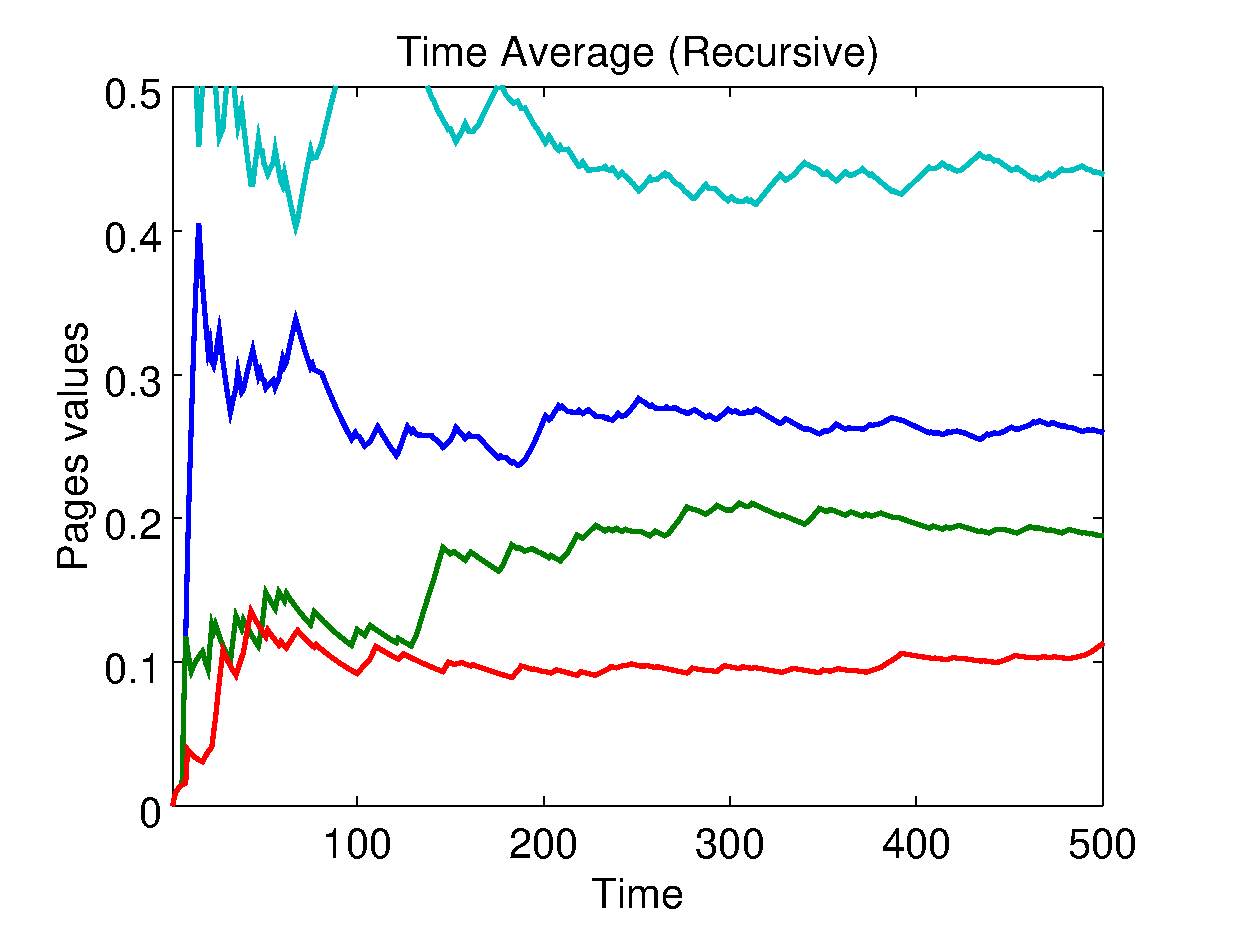
\includegraphics[scale=0.35]{imagens/timerecursive}
	\hspace{0.1cm}
	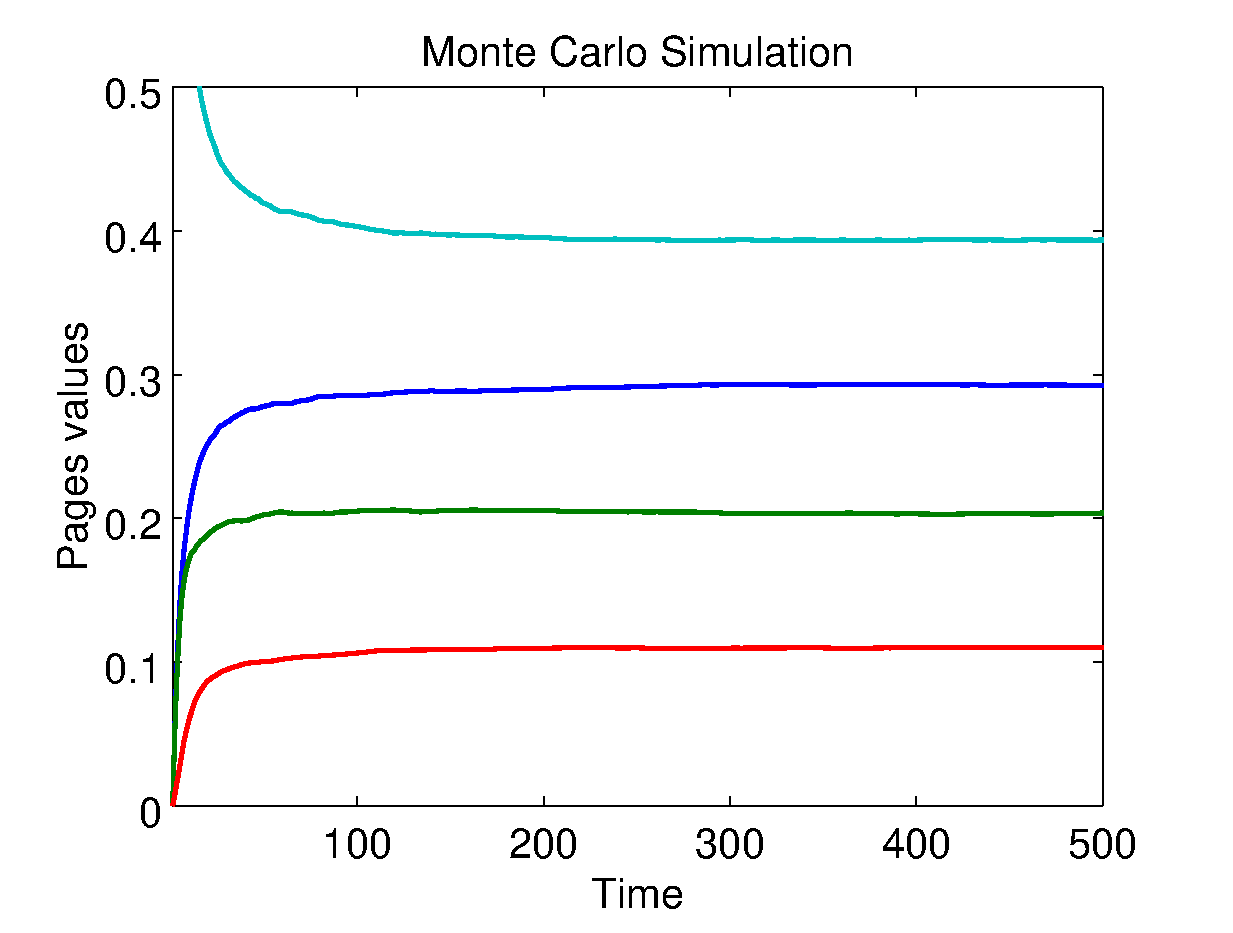
\includegraphics[scale=0.35]{imagens/montecarlo}
	\caption{Comparação entre a média no tempo do modelo distribuído e o método de Monte Carlo.}
	\label{timemonte}
\end{figure}

E ainda comparando os resultados da simulação com Monte Carlo e da simulação do \textit{Power Method} \ref{powermonte}, nota-se que os valores finais estão de acordo com os alcançados no modelo do \textit{Power Method}, o que sugere que o modelo é válido.

\
\begin{figure}[!htb]
	\centering
	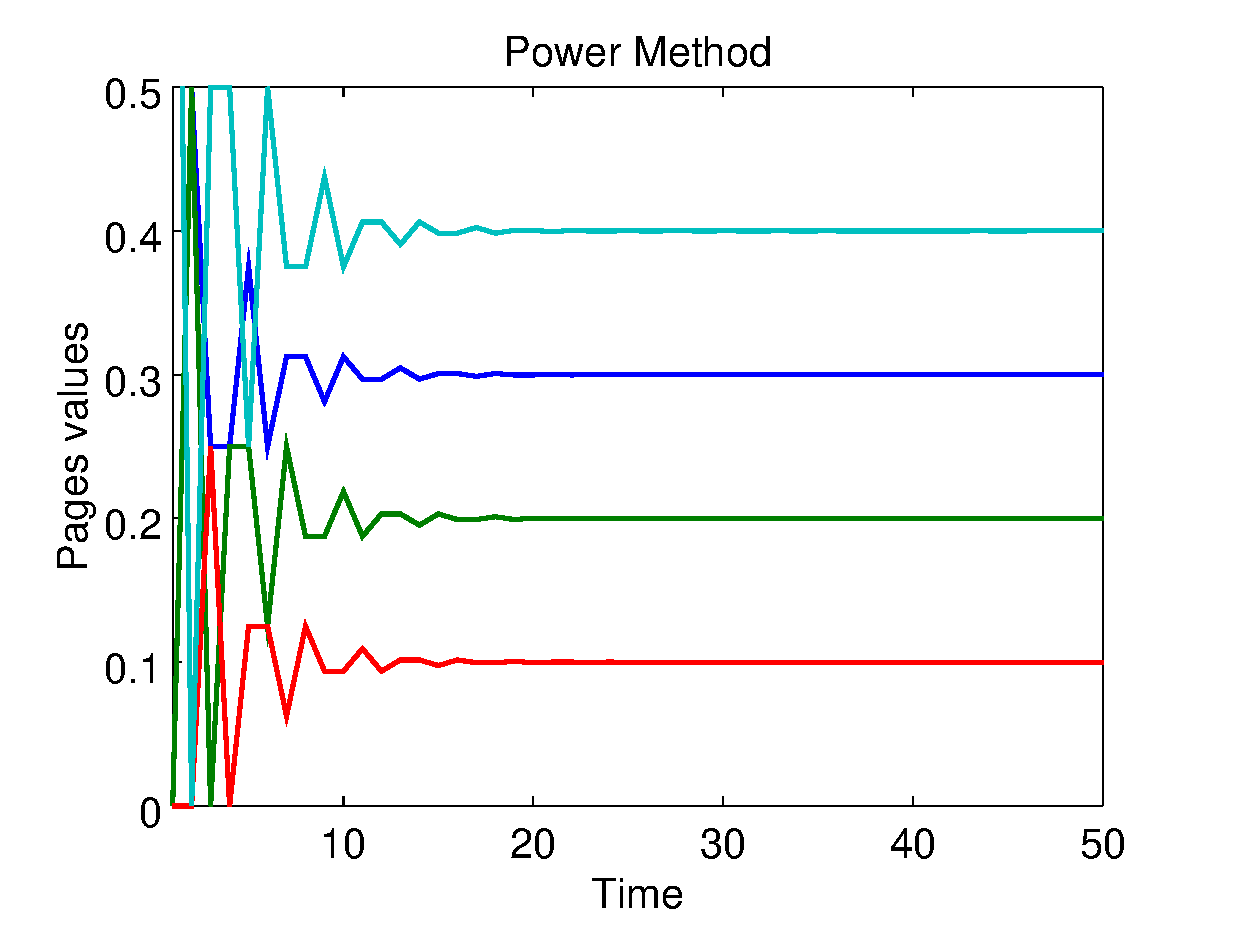
\includegraphics[scale=0.35]{imagens/powermethod}
	\hspace{0.1cm}
	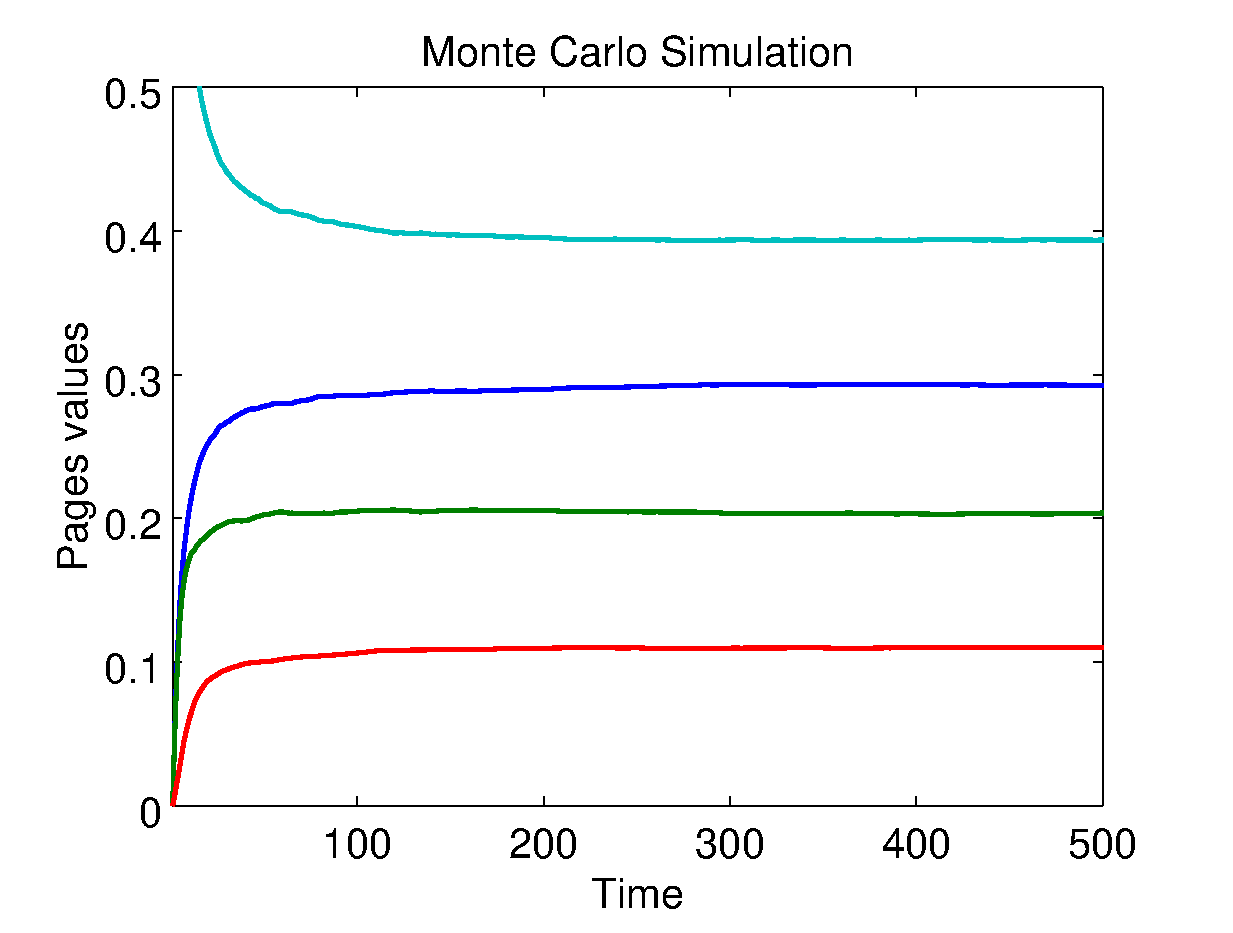
\includegraphics[scale=0.35]{imagens/montecarlo}
	\caption{Comparação entre os resultados do \textit{Power Method} e os obtidos com o método de Monte Carlo.}
	\label{powermonte}
\end{figure}
%%%%%%%%%%%%%%%%%%%%%%%%%%%%%%%
\chapter{Considerações Finais}%
%%%%%%%%%%%%%%%%%%%%%%%%%%%%%%%

%Retornar o assunto principal.
Desde o início das pesquisas em desenvolvimento de ferramentas de busca em 1994, conseguir fazer um ranqueamento de páginas \textit{Web} de acordo com os interesses do usuário tem sido a parte mais desafiadora no desenvolvimento desses sistemas. Foi talvez por partir desse problema, e com uma boa solução, que o buscador Google obteve tamanho sucesso desde sua criação ao final da década de 90. As técnicas e modelos por trás do ranqueamento desse conjunto de documentos foram publicadas e, desde então, a comunidade científica tem trabalhado na pesquisa de novos modelos para tornar o cálculo do \textit{PageRank} mais eficiente.

O cálculo do \textit{PageRank} pode ser representado por diversos modelos, mas de forma geral é apresentado como uma equação de diferença, com algumas modificações na matriz de transição, a fim de tratar possíveis problemas de convergência. Os modelos e as propostas mais recentes do algoritmo estão voltados para o problema da distribuição do cálculo do ranquemento, no intuito de torná-lo cada vez mais eficiente. Mas a atenção ao algoritmo não tem por fim somente o ranqueamento de páginas \textit{Web}, a ideia do cálculo do \textit{PageRank} pode ser aplicada a diversos outros problemas.

%O que conclui-se do trabalho, objetivo geral e contribuições. Porque o meu trabalho é importante?
Durante o trabalho foi realizada uma revisão dos modelos propostos para o algoritmo do \textit{PageRank} na literatura. De forma que, inicialmente fosse efetuado um estudo dos modelos matemáticos por trás do algoritmo e em seguida fossem realizadas as simulações. Também para que fossem compreendidos os modelos matemáticos por trás do algoritmo, foi realizado um estudo sobre questões relacionadas a sistemas dinâmicos, sistemas estocásticos e probabilidade. %Pode-se então adquirir bastante conhecimento com a revisão desses assuntos e com as análises feitas a partir dos resultados. 

%Indicar trabalhos futuros a serem desenvolvidos.
Neste trabalho ainda pretende-se utilizar outros métodos válidos na simulação do \textit{PageRank}. Como a cada ano novos artigos são publicados no tema, novos modelos e técnicas estão sempre sendo publicados pela comunidade científica. Porém uma atenção maior seria dada a modelos agregados de cadeias de Markov, e problemas de consenso. E ainda como uma continuação deste trabalho, poderia ser feita uma implementação com \textit{links} já coletados por um \textit{Web Crawling}. De forma a por em prática os modelos num ambiente real e usando-se de técnicas de computação distribuída, afim de otimizar o cálculo e por em prática os algoritmos distribuídos. Além de usar outras linguagens de programação, como C e C++, por questões de desempenho e por serem mais adequadas a implementações em \textit{clusters}.
%%%%%%%%%%%%%%%%%%%%%
\chapter*{Apêndices}%
%%%%%%%%%%%%%%%%%%%%%


%%%%%%%%%%%%%%%%%%%%%%%%%%%%%%%%%%%%%%%%%%%%%%%%%%%%%%%%%%%%%%%%%%%%%%%%%%%%%%%%%%%%%%%
\section*{Apêndice A - Dedução do Modelo Recursivo da Média no Tempo}\label{apendiceA}%
%%%%%%%%%%%%%%%%%%%%%%%%%%%%%%%%%%%%%%%%%%%%%%%%%%%%%%%%%%%%%%%%%%%%%%%%%%%%%%%%%%%%%%%

Partindo-se da equação da média no tempo \eqref{y}, e fazendo-se um avanço de uma iteração no vetor da média, tem-se:

\begin{equation}\nonumber
y(k) = \frac{1}{k+1} \sum^{k}_{l=0} x(l)
\end{equation}

\begin{equation}\nonumber
y(k+1) = \frac{1}{k+2} \sum^{k+1}_{l=0} x(l)
\end{equation}

\begin{equation}\nonumber
y(k+1) = \frac{1}{k+2} [x(0) + x(1) + ... + x(k) + x(k+1)]
\end{equation}

\begin{equation}\nonumber
y(k+1) = \frac{1}{k+2} \sum^{k}_{l=0} x(l) + \frac{1}{k+2} x(k+1)
\end{equation}

\begin{equation}\nonumber
y(k+1) = \frac{1}{k+2} (k+1)y(k) + \frac{1}{k+2} x(k+1)
\end{equation}\\

Por fim, o método recursivo da média no tempo é dado pela seguinte equação:

\begin{equation}\nonumber
y(k+1) = \frac{k+1}{k+2} y(k) + \frac{1}{k+2} x(k+1)
\end{equation}\\

Esta equação segue o mesmo formato da apresentada em \eqref{yr}.


%%%%%%%%%%%%%%%%%%%%%%%%%%%%%%%%%%%%%%%%%%%%%%%%%%%%%%%%%%%%%%%%%%%%%%%%%%%%%%%%%%%%%%%%%
\section*{Apêndice B - Código em Linguagem MATLAB Usado nas Simulações}\label{apendiceB}%
%%%%%%%%%%%%%%%%%%%%%%%%%%%%%%%%%%%%%%%%%%%%%%%%%%%%%%%%%%%%%%%%%%%%%%%%%%%%%%%%%%%%%%%%%

\lstinputlisting{apendice/pagerank.m}

%===================================================================================
%\backmatter
%===================================================================================

%\bibliography{monografia}{}
%\bibliographystyle{abnt-alf}

% OUTRA FORMA DE CRIAR A BIBLIOGRAFIA:
\bibliographystyle{plain}
\bibliography{ref}


\anexo
\end{document}